% main.tex - Updated Research Template with new title page
\documentclass{research}

\usepackage{graphicx} %LaTeX package to import graphics
\graphicspath{{images/}} %configuring the graphicx package

\usepackage{ragged2e} % Add this to your preamble

% Title Page Info
\title{}
\author{Fritzgerald Enric T. Imperial}
\submission{A Special Project Presented to the Faculty of the College of Computer Studies, Naga College Foundation, Inc., Naga City}
\researchyear{2026}

\usepackage{float}
\usepackage{longtable}
\usepackage{amsmath}      % REQUIRED for equation*, \Sigma, \times, \frac
\usepackage{amssymb}      % for math symbols
\usepackage{enumitem}     % for custom list labels
\usepackage{booktabs} % Required for professional horizontal rules
\usepackage{caption}  % For proper spacing between caption and table
\usepackage{array}
\usepackage{indentfirst}

\graphicspath{{./}{./figures/}}

\begin{document}

% Generate Title Page
\thispagestyle{empty}
\begin{center}
  \vspace*{1in}
  {\Huge\bfseries E-Health for All: A User-Centered Telemedicine System \par}
  \vspace{1in}
  A Capstone Project\\
  Presented to the Faculty of the\\
  College of Computer Studies\\
  Naga College Foundation, Inc.\\
  Naga City\\
  \vspace{1in}
  In Partial Fulfillment of\\
  The Requirements for the Degree\\
  Bachelor of Science in Information System\\
  \vspace{0.5in}
  Ian V. Bruzo\\
  Dominica SL. Narvato\\
  Kristine Carla I. Paraiso\\
  EJ Andrei J. Villamer\\
   \vspace*{0.8in}
  2027
\end{center}

\clearpage

\tableofcontents

\clearpage

\listoffigures

\clearpage

\listoftables

\clearpage

\clearpage

%-----------------------------
% Chapter 1
%-----------------------------
\chapter{Introduction}

\section{Background of the Study}

Healthcare access remains one of the most persistent global inequalities, with limited specialist availability and inadequate infrastructure keeping millions from critical care. The World Health Organization estimates that half of the global population lacks access to essential health services, with rural communities disproportionately affected \cite{ref66}, leading to delayed diagnoses and preventable deaths. Telemedicine presents a promising solution by delivering healthcare across distances, connecting remote patients with specialists without requiring travel and making scarce resources available to underserved populations.

In the Philippines, these challenges are especially severe. The country's geography and urban concentration of medical specialists leave rural populations with limited healthcare options. In response, the Philippine government and health institutions have begun embracing telemedicine to broaden coverage. The National Telehealth Center has launched SMS and web-based platforms connecting rural patients with specialist consultations \cite{ref25}, \cite{ref59}, and various health institutions have adopted electronic medical records to improve continuity of care across facilities \cite{ref36}, \cite{ref40}.

Despite these efforts, significant barriers persist. Poor transportation infrastructure hinders facility access, particularly during emergencies and follow-up care. Unreliable internet connectivity, limited computing resources, and low digital literacy among both patients and healthcare workers further compound these challenges \cite{ref1}, \cite{ref46}. Existing telemedicine initiatives, while promising, remain fragmented and rarely address the unique technological constraints and cultural context of rural Filipino communities \cite{ref49}, \cite{ref51}.

This research seeks to bridge these gaps by developing an integrated telemedicine platform specifically designed for the selected rural barangays. The platform combines three components, a comprehensive doctors' database, a patient records management system, and an appointment scheduling system into one user-friendly interface accessible to users with different levels of digital literacy. 

This initiative aligns with multiple UN Sustainable Development Goals: good health and well-being (sdg3), by improving healthcare access and quality. It supports industry, innovation, and infrastructure (sdg9), by demonstrating how technology can address healthcare infrastructure gaps in underserved areas. It advances reduced inequalities (sdg10), by examining how digital health solutions reduce disparities in healthcare access across different populations and socioeconomic groups.

\section{Review of Related Literature}

\subsection*{Telemedicine Adoption and Implementation }

Telemedicine, the delivery of healthcare services using information and communication technologies, has emerged as a vital solution for healthcare access issues in isolated and underserved communities. Telemedicine allows healthcare providers to assess, diagnose, and treat patients in remote areas by utilizing telecommunications technology to effectively connects medical experts with populations that have limited access to healthcare facilities. It has shown great promise in overcoming healthcare access issues in rural communities around the world. 

Research shows that telemedicine consultations promote better clinical decision-making, reduce unnecessary patient transfers, and increase the chances of local admissions instead of costly transfers to far-off hospitals \cite{ref30}, \cite{ref27}. These advantages apply to many medical fields, from primary care to specialized areas like neurology and emergency medicine \cite{ref15}.

However, the pandemic highlighted the shortcomings of telemedicine: access services at lower rates \cite{ref10},\cite{ref21}. Digital literacy among older adults and low-income individuals \cite{ref1},\cite{ref46}, equal access concerns \cite{ref16},\cite{ref12},\cite{ref6}, implementation costs and maintenance \cite{ref43},\cite{ref9}, infrastructure issues \cite{ref31},\cite{ref48},\cite{ref62}., and data security and patient privacy concerns \cite{ref41}.

On the one hand, communities with integrated systems achieve better health outcomes for managing chronic diseases compared to those that use fragmented record-keeping \cite{ref32}. Patient satisfaction with telemedicine in the Philippines shows encouraging trends \cite{ref32},\cite{ref39}. Even senior citizens, increasingly accepted remote consultations \cite{ref7}. The University of the Philippines Health Service successfully used tailored electronic medical records systems in various settings during COVID-19, ensuring continuity of patient care despite mobility restrictions \cite{ref36},\cite{ref59}. Thorough assessments show considerable progress in adoption over time, although significant gaps between different types of facilities and locations persist \cite{ref3},\cite{ref38}.

Successfully implementing telemedicine requires careful adjustments to local circumstances. Detailed analyses reveal Philippines-specific barriers like governance issues, unclear licensure requirements, unresolved liability problems, and vague reimbursement mechanisms that hinder healthcare provider involvement \cite{ref25},\cite{ref51}. Healthcare technology must consider local cultural practices, language preferences, and health-seeking behaviors to ensure meaningful user acceptance in diverse Filipino communities \cite{ref49}. Creating user-friendly systems is crucial for sustained adoption rather than leaving behind abandoned pilot projects \cite{ref63}. 

\subsection*{Patient Information Management System }
Patient information management involves the organized collection, storage, and use of health data to support clinical decision-making and ensure continuity of care. Electronic Medical Records (EMR) systems digitize patient health information, enabling providers to access complete histories, track treatments, identify medication interactions, and coordinate care across specialties. This is especially critical in rural and underserved areas where access to prior care records is limited.

EMR systems significantly improve care coordination, with integrated communities achieving better chronic disease outcomes compared to those with fragmented records \cite{ref33}, \cite{ref19}. However, while basic adoption rates are high, comprehensive implementation remains lower in rural facilities despite recognized benefits \cite{ref12}, \cite{ref6}. Technical, organizational, and workflow barriers continue to hinder smooth information sharing \cite{ref48}, \cite{ref3}, \cite{ref38}, and digital literacy gaps among older adults and low-income individuals require targeted design and training interventions \cite{ref1}.

Data security and patient privacy are foundational to EMR trust, requiring encryption, access controls, and audit trails \cite{ref41}. Integrated systems reduce administrative burdens and improve care delivery \cite{ref45}, \cite{ref56}, \cite{ref26}, while predictive models using patient data enable targeted interventions and better resource allocation \cite{ref17}, \cite{ref13}, supporting a shift toward proactive, preventive primary care \cite{ref11}.

In the Philippines, EMR adoption shows both progress and challenges. COVID-19 visibly impacted system usage in rural health facilities \cite{ref2}, yet implementation improved clinical decision-making and reduced medication errors compared to paper systems \cite{ref40}. Sustained adoption is linked to training, technical support, and gradual workflow integration rather than rapid rollouts \cite{ref28}, though research representation across specialties, settings, and facility types remains uneven \cite{ref14}. The absence of centralized provider databases causes referral delays and disjointed care \cite{ref60}, while comprehensive physician databases with specialization and scheduling details enhance diagnostic workflows \cite{ref53}. Keeping such databases accurate remains challenging, necessitating automated verification and validation processes \cite{ref35}.

\subsection*{Appointment Scheduling in Healthcare }
Appointment scheduling systems are essential to healthcare delivery, coordinating patient needs, provider availability, and facility resources. Well-designed systems reduce waiting times, lower missed appointments through automated reminders, improve provider productivity, and ensure urgent cases receive prompt attention. In rural settings, where patients face long travel distances and transportation barriers, efficient scheduling is especially critical for maintaining access and treatment adherence.

Digital scheduling significantly reduces no-show rates compared to offline booking, with automated reminders proving particularly effective \cite{ref45}. AI-driven tools further improve efficiency by predicting non-attendance and optimizing resource allocation \cite{ref56}, while open-access scheduling reduces no-shows by offering same-day or next-day appointments \cite{ref26}. Predictive models incorporating patient demographics and appointment history identify high lead time and prior missed appointments as the strongest predictors of non-attendance \cite{ref17}, \cite{ref13}. Integrated systems also improve patient flow and reduce waiting area congestion in underserved facilities \cite{ref65}, supporting broader proactive primary care initiatives through timely referrals and fewer missed appointments \cite{ref11}, \cite{ref35}.

In the Philippines, digital appointment management in rural health centers has shortened waiting times and reduced missed appointments through better time slot management and automated reminders \cite{ref50}. However, rural contexts require flexible approaches, as rigid scheduling is ineffective where patients face unreliable transportation or inflexible work schedules. Systems must therefore incorporate easy rescheduling options and reminder methods that function without internet access \cite{ref37}.

\section{Synthesis of the State-of-the-Art }
The detailed collection of works and studies offered valuable insights into the topic. These studies backed their claims with relevant data and detailed information. This section will provide a brief overview of the reviews of relevant literature.

Telemedicine has emerged as a viable solution to geographic barriers, improving clinical decision-making, reducing unnecessary transfers, and expanding specialist access \cite{ref15}, \cite{ref30}, \cite{ref27}. However, persistent challenges remain, including infrastructure limitations, digital literacy gaps, data security concerns, and Philippines-specific barriers such as unclear licensure, liability, and reimbursement mechanisms \cite{ref25}, \cite{ref41}, \cite{ref46}, \cite{ref51}. Despite these, large-scale pilots in the Philippines demonstrate feasibility across diverse communities, with patient satisfaction showing encouraging trends even among senior citizens \cite{ref7}, \cite{ref32}, \cite{ref39}, \cite{ref59}. Successful adoption requires culturally sensitive, user-centered design tailored to local contexts \cite{ref49}, \cite{ref63}.

Patient information management systems significantly improve care coordination and clinical outcomes, yet comprehensive EMR implementation remains lower in rural facilities \cite{ref6}, \cite{ref12}. Workflow barriers, digital literacy gaps, and data security concerns continue to hinder full adoption \cite{ref1}, \cite{ref3}, \cite{ref38}, \cite{ref41}. In the Philippines, gradual integration supported by training and technical assistance yields better sustained adoption \cite{ref28}, while the absence of centralized provider databases causes referral delays and fragmented care \cite{ref53}, \cite{ref60}.

Appointment scheduling systems directly reduce no-show rates, improve patient flow, and support proactive primary care \cite{ref11}, \cite{ref45}, \cite{ref56}. Predictive modeling and AI-driven tools further optimize resource allocation \cite{ref17}, \cite{ref13}, \cite{ref56}. In Philippine rural health centers, digital scheduling has measurably shortened waiting times \cite{ref50}, though flexible, offline-capable systems are essential given transportation and connectivity constraints \cite{ref37}.

Across all three areas, the literature consistently points to the need for an integrated, context-sensitive platform that unifies patient records, provider information, and appointment scheduling precisely the gap this research addresses. 

\section{Gap Bridged by the Study}
This study addresses important gaps in rural healthcare delivery by creating an integrated telemedicine platform specifically for rural barangays in Naga City. The reviewed literature reveals that telemedicine adoption, patient information management, and appointment scheduling have largely been studied and addressed as separate concerns rather than as an interdependent system of rural healthcare delivery. Telemedicine adoption in the Philippines have concentrated on broad institutional and policy barriers unclear licensure, liability, and reimbursement mechanisms [2], [9] while comparatively little attention has been given to how these barriers manifest at the level of an individual rural health unit's daily operation.

Similarly, on patient information management establishes that comprehensive EMR implementation remains consistently lower in rural facilities than in urban ones, and attributes this gap to technical, organizational, and workflow barriers [16], [17], [21], [27], [28]. However, these studies tend to evaluate record-keeping systems in isolation, with limited examination of how record management interacts with, or is constrained by, the absence of centralized, verified provider databases has been identified as a distinct cause of referral delays and disjointed care [41], [42], [43], yet this issue is typically treated as a standalone informatics problem rather than as part of a single integrated workflow.

Studies confirm that digital scheduling reduces no-show rates and improves patient flow [32], [33], [34], [44], and that Philippine rural health centers specifically benefit from better time-slot management and automated reminders [45] particularly under the unreliable connectivity conditions documented across rural Philippine settings [9], [46].

Taken together, the literature demonstrates that while telemedicine adoption, patient records management, and appointment scheduling have each been examined and shown to improve outcomes as individual interventions, none of the reviewed studies examine these three components as a single, interdependent system evaluated within one rural Philippine barangay setting. Studies that do call for culturally sensitive, user-centered design [8], [29] stop short of testing this design principle across all three functions simultaneously, and none account concurrently for the specific operational and connectivity constraints of a barangay-level health unit such as Panicuason. This absence of an integrated, empirically grounded, and context-specific examination of rural healthcare workflows constitutes the gap this study addresses

\section{Theoretical Framework}

This study is anchored on the following theories: the Task Technology Fit (TTF) Theory by Goodhue and Thompson, as cited by Thanthrige et al. \cite{ref69}; the Diffusion of Innovations (DOI) Theory by Rogers, as cited by Tsogbe et al. \cite{ref70}; and the Technology Acceptance Model (TAM) by Davis, as cited by Holtz et al. \cite{ref71}.   

\begin{figure}[H]
    \centering
    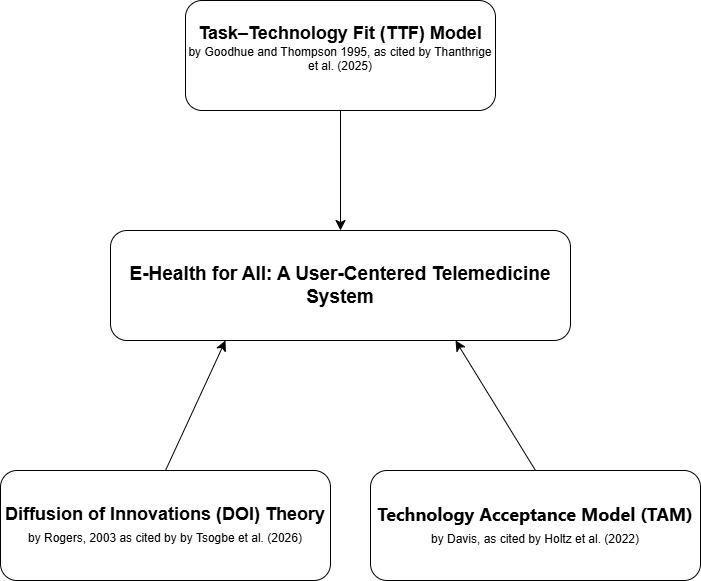
\includegraphics[
        height=0.5\textheight,
        keepaspectratio
    ]{Theoretical_Paradigm}

    \caption{Theoretical Framework}
\end{figure}
The diagram illustrates the theoretical foundations guiding the development of the E-Health for All telemedicine system for improving access in rural communities. Goodhue and Thompson (1995) established that technology is most effectively utilized when its capabilities align with the tasks users must perform. Thanthrige et al. \cite{ref69} reinforced this principle in a 2025 systematic review, confirming that task-technology alignment remains a critical determinant of healthcare technology adoption. This theory anchors the study by evaluating whether the three core features of E-Health for All digital patient records management, automated health worker scheduling, and online appointment booking fit the actual daily tasks of Panicuason health facility personnel, as a technically sound system that lacks this fit will be underused or abandoned.

Rogers (2003) argued that technology adoption is shaped by five key attributes: relative advantage, compatibility, complexity, trialability, and observability. Tsogbe et al. \cite{ref70} applied this framework in 2026 within a telehealth adoption context in a developing-region setting, affirming its continued relevance in guiding digital health implementation. This theory guides the study by ensuring that the E-Health for All platform offers a clear operational advantage over the current paper-based system while remaining compatible with the existing workflows of Barangay Panicuason.

Davis (1989) proposed that technology adoption is primarily driven by perceived usefulness the degree to which a system improves work performance and perceived ease of use the degree to which it is free of effort. Holtz et al. \cite{ref71} applied TAM in 2022 specifically to telemedicine adoption among rural populations, affirming its applicability in this context. This theory directly shapes the acceptability evaluation instrument of the study by measuring whether health facility personnel perceive E-Health for All as useful, easy to use, and trustworthy enough to adopt.

\section{Conceptual Framework}
The Input-Process-Output (IPO) Framework, added with Feedback loop as the fourth component, is the approach utilized in the conceptualization of this study.

\begin{figure}[H]
    \centering
    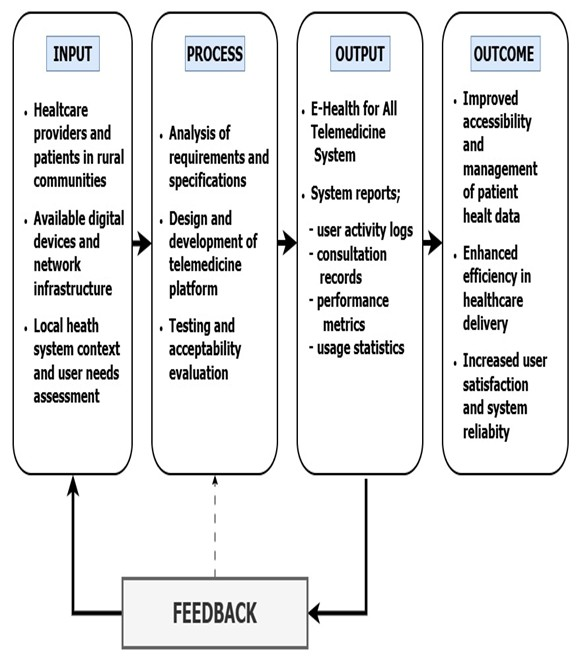
\includegraphics[
        height=0.5\textheight,
        keepaspectratio
    ]{ConceptualParadigm}

    \caption{Conceptual Framework}
\end{figure}
The enhanced system paradigm is the approach utilized in the conceptualization of this study. The input came from various sources to gain a complete understanding of rural healthcare needs and readiness for technology, such as document analysis of health records, observations of healthcare-seeking behaviors and travel times, surveys on evaluating user satisfaction and technology skills, and interviews gathering in-depth information about access challenges and provider readiness for telemedicine services. The processes involved includes, systems analysis and specification for system design, functional testing to ensure adherence to system requirements, usability testing to ensure the system meets the user needs, and acceptability evaluation to validate the system feasibility for deployment. The studys output is a web application with the following features like computer vision, security, authentication, verification, patient check-up history, Qr code security, by using the system it is expected to improve efficiency, achieve fewer documentation and smoother, admin   shorter waiting times, through better appointment, enhance user satisfaction, and improve data security of patient information. The continues feedback mechanism will ensure iterative refinement of the system to remain user friendly, operational and align with rural healthcare. 

\section{Statement of the Problem}

This study aims to address the problem of healthcare accessibility among rural populations. Specifically, this study seeks to answer the following questions:

\begin{enumerate}

    \item What are the current practices of rural healthcare providers in rural populations with respect to:
    \begin{enumerate}
        \item Patient records management
        \item Doctor scheduling
        \item Appointment systems
    \end{enumerate}

    \item What are the challenges encountered in the current system with respect to:
    \begin{enumerate}
        \item Patient records management
        \item Doctor scheduling
        \item Appointment systems
    \end{enumerate}

    \item What system can be designed to address the challenges encountered?

    \item What is the level of acceptability of the system in terms of:
    \begin{enumerate}
        \item Usability
        \item Reliability
        \item Data security
    \end{enumerate}

\end{enumerate}

\section{Assumptions}
This research study is anchored on the following key assumptions:

\begin{enumerate}

    \item Rural healthcare providers in Panicuason, Naga City have specific practices for managing patient records, scheduling doctors, and handling appointments.

    \item There are challenges with the current systems for managing patient records, scheduling doctors, and setting up appointments in rural healthcare facilities.

    \item A user-centered telemedicine platform can be designed and developed to address these challenges in the current healthcare delivery system.

    \item Rural healthcare providers and clinic staff are willing to transition from the current manual practices to the proposed user-friendly telemedicine platform and digital records management system.

\end{enumerate}

\section{Scope and Delimitation}

This study covered the design, development, and initial acceptability evaluation of the E-Health for All telemedicine platform for Barangay Panicuason Rural Health Unit in Naga City, Camarines Sur. The prototype included digital patient health profiles, clinical encounter documentation, vital signs monitoring, medication tracking, appointment booking, automated scheduling, virtual consultation, offline synchronization, prescription scanning, a patient portal, and an integrated health worker database.

The study involved two respondent groups. The 13 health facility personnel of the Panicuason Rural Health Unit, selected through total enumeration, served as respondents for documenting current practices and operational challenges, comprising Dental Health Workers, a Midwife, an Encoder, a Barangay Nutrition Scholar, a Community-Based Rehabilitation Specialist, and a Barangay Social Welfare Aide. A minimum of 80 rural residents of Barangay Panicuason who have direct experience accessing the health facility served as the primary respondents for assessing user needs and evaluating the acceptability of the proposed system, consistent with the study's user-centered focus. Data were gathered through surveys, interviews, observation, and document analysis of existing health records.

The study was delimited to Barangay Panicuason and did not cover other health facilities, long-term system performance, cost-effectiveness, or sustainability of adoption. Laboratory integration, referral system interoperability, billing, and pharmacy management were also excluded, as these fall outside the study's three core areas. External factors such as internet connectivity, power interruptions, and respondents' digital literacy were acknowledged as relevant but were not measured or controlled for in this study.

\section{Significance of the Study}

This study benefits the following stakeholders in advancing rural healthcare delivery and digital health innovation:

\textbf {Patients in Rural Communities}. Rural residents gain access to healthcare services without costly travel, reducing time and financial burdens while ensuring continuity of care for chronic conditions.

\textbf {Rural Healthcare Providers}. Healthcare providers benefit from automated records management, streamlined appointment scheduling, and simplified specialist referrals, enabling more efficient and accurate patient care.

\textbf {Community Health Workers.} Frontline healthcare workers gain faster access to patient information, reducing paperwork and allowing greater focus on direct care, remote consultations, and early detection of emerging health trends.

\textbf {Health Administrators and Local Government Officials.} Administrators gain data-driven insights into service utilization, disease prevalence, and resource allocation, along with a replicable model for digital health initiatives in underserved communities.

\textbf {Technology Developers.} Developers gain practical, evidence-based insights into building offline-capable and low-bandwidth healthcare systems designed for users with limited digital literacy.

\textbf {Academic Researchers.} The study provides validated frameworks and tools for designing context-sensitive digital health solutions, addressing existing research gaps on integrated telemedicine platforms in resource-limited environments.

\section{Definition of Terms}

This section provides clear and precise definitions of key terms used throughout the study, both conceptually and operationally.

\textbf {E-health.} E-health refers to the use of information and communication technologies in healthcare delivery, including telemedicine, electronic medical records, and digital health platforms \cite{ref66}. In this study, it encompasses all electronically delivered health services through the proposed telemedicine platform for rural communities.

\textbf {E-health for All.} E-health for All is a principle that advocates equal access to digital health technologies regardless of location, income, or technical ability \cite{ref20}. In this study, it refers to the commitment to developing inclusive and user-friendly telemedicine solutions for rural communities in Naga City.

\textbf {Telemedicine.} Telemedicine is the delivery of healthcare services and clinical information through communication technologies to overcome geographical barriers \cite{ref24}. In this study, it refers to the proposed remote healthcare delivery system developed for Naga City.

\textbf {User-Centered Design.} User-centered design is a development methodology that focuses on the needs, preferences, and limitations of end-users throughout the design process \cite{ref55}. In this study, it refers to the participatory design approach used in developing the telemedicine platform.

\textbf {Rural Healthcare.} Rural healthcare refers to the provision of medical services in isolated or underserved areas with limited infrastructure and specialist access \cite{ref47}. In this study, it refers to healthcare delivery in rural barangays of Naga City.

\textbf {Telehealth Platform}. A telehealth platform is a digital healthcare ecosystem integrating provider directories, patient information systems, and scheduling tools to facilitate remote healthcare delivery \cite{ref61}. In this study, it refers to the web-based system developed for Naga City.

\textbf {Healthcare Accessibility.} Healthcare accessibility refers to the ease with which individuals obtain necessary health services considering physical, geographical, economic, and organizational factors. In this study, it refers to how rural residents of Naga City access healthcare services through the proposed telemedicine platform.


\clearpage

%-----------------------------
% Chapter 2
%-----------------------------
\chapter{Methodology}

This section outlines the research methodology. It covers the research design, participants, location, data collection methods and tools, ethical considerations, statistical analysis, project timeline, and validation methods to ensure the reliability of the findings.

\section{Research Design}
This study adopted a developmental-descriptive research design to document current healthcare practices, identify operational challenges, and develop a telemedicine solution suited to the needs of Barangay Panicuason RHU. Data were collected through surveys, interviews, observations, and document analysis, following four phases: preparation, assessment, data collection, and analysis.

\section{Population and Sampling}
This study involved two respondent groups. The first group comprised the 13 health facility personnel of Barangay Panicuason Rural Health Unit, selected through total enumeration as the primary end-users responsible for patient records management, health worker scheduling, and appointment handling. This group consisted of 7 Dental Health Workers, 1 Midwife, 1 Encoder, 1 Barangay Nutrition Scholar (BNS), 1 Supplemental Feeding Volunteer (SFV), 1 Community-Based Rehabilitation Specialist (CBRS), and 1 Barangay Social Welfare Aide (BSWA). Total enumeration was used for this group given the small and clearly defined population of facility personnel, allowing the study to capture data from all individuals directly responsible for the current manual processes under investigation.

The second group comprised rural resident-users of Barangay Panicuason, included as co-primary respondents consistent with the study's user-centered focus. This group was selected through purposive sampling, limited to residents with direct experience accessing the barangay health facility, since the study required respondents who could meaningfully evaluate the system's relevance to their actual healthcare-seeking behavior rather than a random cross-section of the general population. A minimum sample size of 80 respondents was targeted for this group, determined through Slovin's formula based on the barangay's total population.


% ============================================================
% RESEARCH LOCALE
% ============================================================

\subsection{Research Locale}

 The study was conducted at Barangay Panicuason Rural Health Unit in Naga City, Camarines Sur, a barangay situated outside the urban center and characterized
by limited specialist availability, long travel distances to medical facilities, and insufficient healthcare infrastructure. The facility served as the primary healthcare provider for residents of Barangay Panicuason, offering basic services including primary care, maternal and child health, immunization, and disease prevention, and referring cases requiring specialized care to hospitals in Naga City proper.

\subsection{Data Gathering Procedure}

\indent This section describes the methods and tools the researchers used to capture 
data from stakeholders essential to this study.

\indent \textbf{Preparation Phase.} The researchers secured formal permissions from 
barangay officials and local health officers, prepared consent forms, and coordinated 
with community leaders to schedule observation and interview dates within the first 
two weeks.

\indent \textbf{Document Analysis.} The researchers examined health records, referral 
systems, and community health profiles from barangay health stations to document current 
healthcare access patterns and identify existing challenges.

\indent \textbf{Direct Observation.} The researchers observed and recorded how the 
health facility personnel managed patient consultations, handled records, and coordinated 
scheduling and appointments in their actual work setting.

 \textbf{Surveys.} A structured questionnaire was administered to all 13 health 
facility personnel to gather data on current practices, encountered challenges, importance 
of proposed system features, and level of system acceptability.

 \textbf{Interviews.} One-on-one interviews lasting 30 to 45 minutes were 
conducted with the 13 health facility personnel of Barangay Panicuason Rural Health Unit 
to explore current healthcare practices, operational challenges, and readiness for a 
telemedicine solution.

 \textbf{Data Analysis and Documentation.} Survey responses were tallied and 
computed using weighted mean and frequency distribution, while interview data were 
organized by themes and used as the basis for the final findings and recommendations.

\section{Research Instrument}

\indent The study was used various research instruments to collect accurate and relevant data from participants. These instruments are designed to gather both qualitative and quantitative information to gather specific information that will help us understand the current healthcare access situation and identify what is needed for an effective telemedicine platform.

\textbf{Interview Guides.} Researchers will prepare interview guides for rural residents 
of Barangay Panicuason covering healthcare experiences, travel distance to facilities, 
medical costs including transportation, common health problems, mobile and internet 
access, technology comfort level, and desired telemedicine features. For health center 
staff, guides will cover record-keeping systems, data management challenges, internet 
connectivity, available devices, and infrastructure needs. All guides will include 
follow-up questions to explore key points further.

\textbf{Survey Questionnaires.} For healthcare providers and health workers, the 
questionnaire covers demographic profile, years of experience, and current practices 
in patient records management, doctor scheduling, and appointment systems using a 
5-point frequency scale. It also addresses challenges encountered in each of these 
areas, the importance of proposed system features such as digital record storage, 
automated scheduling, online appointment booking, and role-based access control, and 
the perceived level of system acceptability in terms of usability, reliability, and 
data security.

\section{Ethical Considerations}

This research will follow strict ethical guidelines to protect all participants and 
ensure responsible handling of operational data. The following measures will be 
implemented:

\textbf{Voluntary Participation.} Participation was completely voluntary, with no 
pressure or undue incentives influencing the decision to join. Participants may skip 
any question or withdraw at any time without consequences or effect on their access 
to healthcare services.

\textbf{Informed Consent.} All participants received detailed information covering 
the study's purpose, data collection and use, potential risks and benefits, 
confidentiality measures, and the right to withdraw before agreeing to participate. 
Those who agreed signed an informed consent form.

\textbf{Parental/Guardian Consent and Minor Assent.} For participants under 18, 
written parental or guardian consent will be obtained prior to any research 
involvement, and minors aged 7--17 will provide written assent after receiving 
age-appropriate study information. Minors may decline participation even if parents 
have given consent.

\textbf{Consent from Barangay Health Workers (BHWs).} BHWs will sign informed 
consent forms acknowledging permission to collect and use their personal information, 
professional insights, and community health observations. The form will clarify how 
their contributions will be used and ensure their information is protected under 
data privacy regulations.

\textbf{Privacy and Confidentiality.} Individual identities were not revealed without 
explicit written permission, and all interview recordings and transcripts were stored 
in password-protected files accessible only to the research team. Researchers will 
not photograph or record any actual patient medical records containing private health 
information.

\textbf{Data Protection.} All research data will be handled in accordance with the 
Data Privacy Act of 2012 (Republic Act No. 10173), with personal identifiers removed 
and survey responses kept anonymous. All data will be securely destroyed after thesis 
completion and any required retention period.

\textbf{Minimizing Risk.} Research procedures present minimal risk, and researchers 
will travel to participants' communities to reduce inconvenience. If participants feel 
uncomfortable during interviews, sessions will be paused or ended immediately with 
appropriate referrals provided if needed.

\textbf{Cultural Sensitivity.} Researchers will approach all interactions with 
cultural humility and respect for local practices, collaborating with community 
leaders to ensure research activities are culturally appropriate and scheduled at 
convenient times.

\textbf{Researcher Responsibilities.} The research team is committed to accurately 
recording and reporting all data without fabrication or selective omission, properly 
citing all sources, and honestly reporting the research process including challenges 
and limitations. Findings will be shared with participating communities upon request.

\subsection{Statistical Tools}

This section explains how we will analyze and interpret the collected data to answer 
the research questions.

\subsubsection{Descriptive Statistics}

The study employed descriptive statistical methods to summarize and describe the 
characteristics of the sample and their responses. The following descriptive 
statistics were used: percentage, frequency distribution, and weighted mean.

\textbf{Percentage.} To show the proportion of respondents who chose each answer 
option, we will calculate percentages using the formula:

\begin{equation*}
    \text{Percentage} = \frac{f}{N} \times 100
\end{equation*}

\noindent where:
\begin{itemize}[label={}, leftmargin=0pt, itemsep=0pt]
    \item $f$ = frequency or number of responses for a specific option
    \item $N$ = total number of respondents
\end{itemize}

For example, if 45 out of 60 rural residents say they want mobile access to health 
records, the percentage would be calculated as $(45/60) \times 100 = 75\%$.

\textbf{Frequency Distribution.} We will create frequency tables displaying how many 
respondents selected each response option. For instance, for a satisfaction question 
with a 5-point scale, the frequency distribution might be presented as:

\begin{table}[h]
    \centering
    \caption{Frequency Distribution}
    \label{tab:frequency_distribution}
    \begin{tabular}{ccc} % Removed vertical bars (|) for the clean layout
        \toprule
        \textbf{Response Category} & \textbf{Number of Respondents} & \textbf{Percentage} \\
        \midrule % Line sits cleanly below the header row
        Very Satisfied      & 5  & 8.3\%  \\ 
        Satisfied           & 25 & 41.7\% \\ 
        Neutral             & 15 & 25.0\% \\ 
        Dissatisfied        & 10 & 16.7\% \\ 
        Very Dissatisfied   & 5  & 8.3\%  \\
        \textbf{Total}      & \textbf{60} & \textbf{100\%} \\
        \bottomrule % Final closing line at the bottom
    \end{tabular}
\end{table}

\textbf{Weighted Mean.} For Likert-scale items where we want to account for the 
frequency of each response, we will calculate the weighted mean using the formula:

\begin{equation*}
    \text{Weighted Mean} = \frac{\Sigma(W \times f)}{N}
\end{equation*}

\noindent where:
\begin{itemize}[label={}, leftmargin=0pt, itemsep=0pt]
    \item $W$ = weight or scale value (1--5 for a 5-point Likert scale)
    \item $f$ = frequency or number of respondents who chose that value
    \item $N$ = total number of respondents
    \item $\Sigma$ = summation symbol
\end{itemize}

%  \section{Statistical Treatment of Data}

% The data gathered will be interpreted using a five-point Likert scale to measure the respondents' attitudes, opinions, perceptions, and preferences regarding the user-centered telemedicine system. 
	
% Interpretation Scale. To interpret the weighted mean values obtained from Likert-scale questions, the following scale will be used

% \begin{table}[h]
%     \centering
%     \caption{Frequency Distribution}
%     \label{tab:frequency_distribution}
%     \begin{tabular}{lcc} % Removed vertical bars (|) and adjusted alignment for clean look
%         \toprule
%         \textbf{Response Category} & \textbf{Number of Respondents} & \textbf{Percentage} \\
%         \midrule % This line sits directly under the header row
%         Very Satisfied      & 5  & 8.3\%  \\ 
%         Satisfied           & 25 & 41.7\% \\ 
%         Neutral             & 15 & 25.0\% \\ 
%         Dissatisfied        & 10 & 16.7\% \\ 
%         Very Dissatisfied   & 5  & 8.3\%  \\
%         \textbf{Total}      & \textbf{60} & \textbf{100\%} \\
%         \bottomrule % This is the final closing line at the very bottom
%     \end{tabular}
% \end{table}

\section{System Design and Architecture}

The system design process employed several modeling techniques such as use case and system workflows to map user interactions and the system architecture.

\textbf{Technology Stack.} The E-Health for All system was developed using PHP, HTML, CSS, and JavaScript for the web-based platform, with Supabase serving as the cloud database for centralized data storage, authentication, and real-time synchronization. This stack was selected for its low infrastructure overhead and broad compatibility, allowing the system to run on Windows, macOS, and Linux for the web-based platform, and on Android and iOS for the mobile application used by rural residents and health workers in the field.

\textbf{Connectivity Approach.} The system does not resolve the underlying internet infrastructure limitations of Barangay Panicuason actual connectivity conditions in the area remain outside the study's control, as stated in the Scope and Delimitation. What the system does provide is an offline-capable data entry mode on the mobile side, allowing health workers to continue recording patient information, vitals, and consultation notes even when internet access is interrupted. Once connectivity is restored, locally stored records are automatically synced to the central Supabase database. This design mitigates the operational impact of intermittent connectivity on day-to-day recording and access tasks, rather than addressing the broader infrastructure problem of unreliable or absent internet service in the barangay itself.

\subsection*{Use Case}

The use case diagram in the study showed the specific interactions between patients, 
healthcare providers, and system administrators with the system. It defined the actions 
between these actors and the use cases, along with the functional requirements. The use 
case model for this study was shown in Figure~\ref{fig:use_case_diagram}.

In the use case diagram, there were three actors: patients, doctors, and system 
administrators. All actors can register and log in to the system. Patients and doctors 
utilize a mobile application, while system administrators access a dedicated website 
application.

\begin{figure}[H]
    \centering
    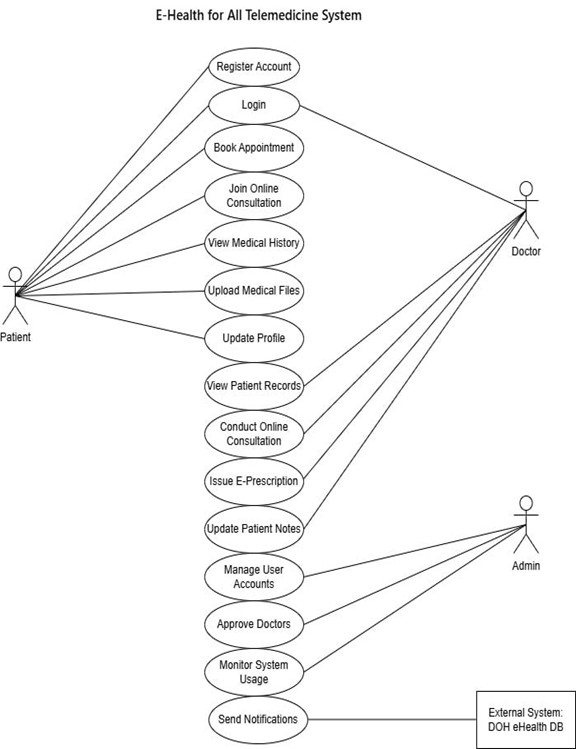
\includegraphics[width=0.80\textwidth]{UseCaseDiagram.jpg}
    \caption{Use Case Diagram}
    \label{fig:use_case_diagram}
\end{figure}

\subsubsection{System Workflows}

The system workflows illustrate the sequential processes and decision points for key operations within the E-Health for All Telemedicine System. These workflows ensure standardized procedures and guide users through various system functionalities.

\begin{figure}[H]
    \centering
    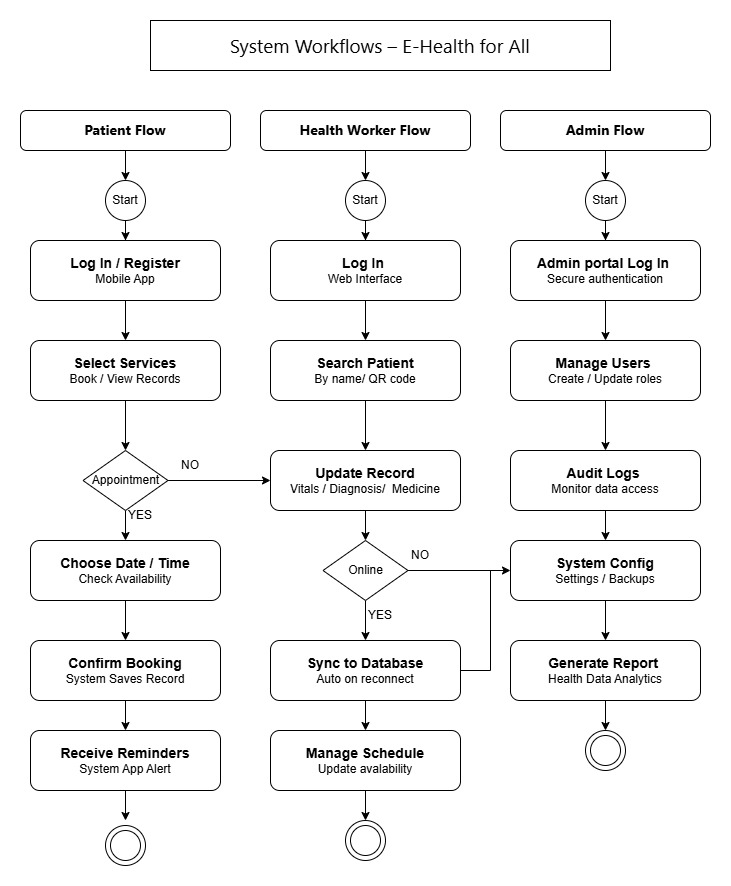
\includegraphics[width=0.85\textwidth]{System_Workflows}
    \caption{System Workflow Diagram}
    \label{fig:workflows}
\end{figure}

\textbf{Patient Flow.} The patient workflow begins with login or registration. After authentication, patients can select services, check appointment availability, choose dates and times, confirm bookings, receive reminders, and complete their system appointments. This streamlined process ensures efficient access to healthcare services.

\textbf{Health Worker Flow.} Health workers log into the web interface, search patients by name or QR code, update medical records, manage diagnosis and prescriptions, sync data to the database, and complete patient consultations. This workflow maintains accurate and up-to-date patient information.

\textbf{Admin Flow.} Administrators access the admin portal through secure authentication, manage users by creating or deactivating accounts, conduct audit log reviews, perform system configuration, generate analytical reports on health data, and monitor overall system performance. These workflows ensure proper governance and system integrity.

\subsubsection{DFD Level 0}

The Context Diagram shows the entire data flow of the E-Health for All Telemedicine System, where four external entities --- Patient, Doctor, BHW, and Admin exchange certain data with the system. This diagram serves as a foundation for designing the system. The data coming into and out of the system is clearly represented.

\begin{figure}[H]
    \centering
    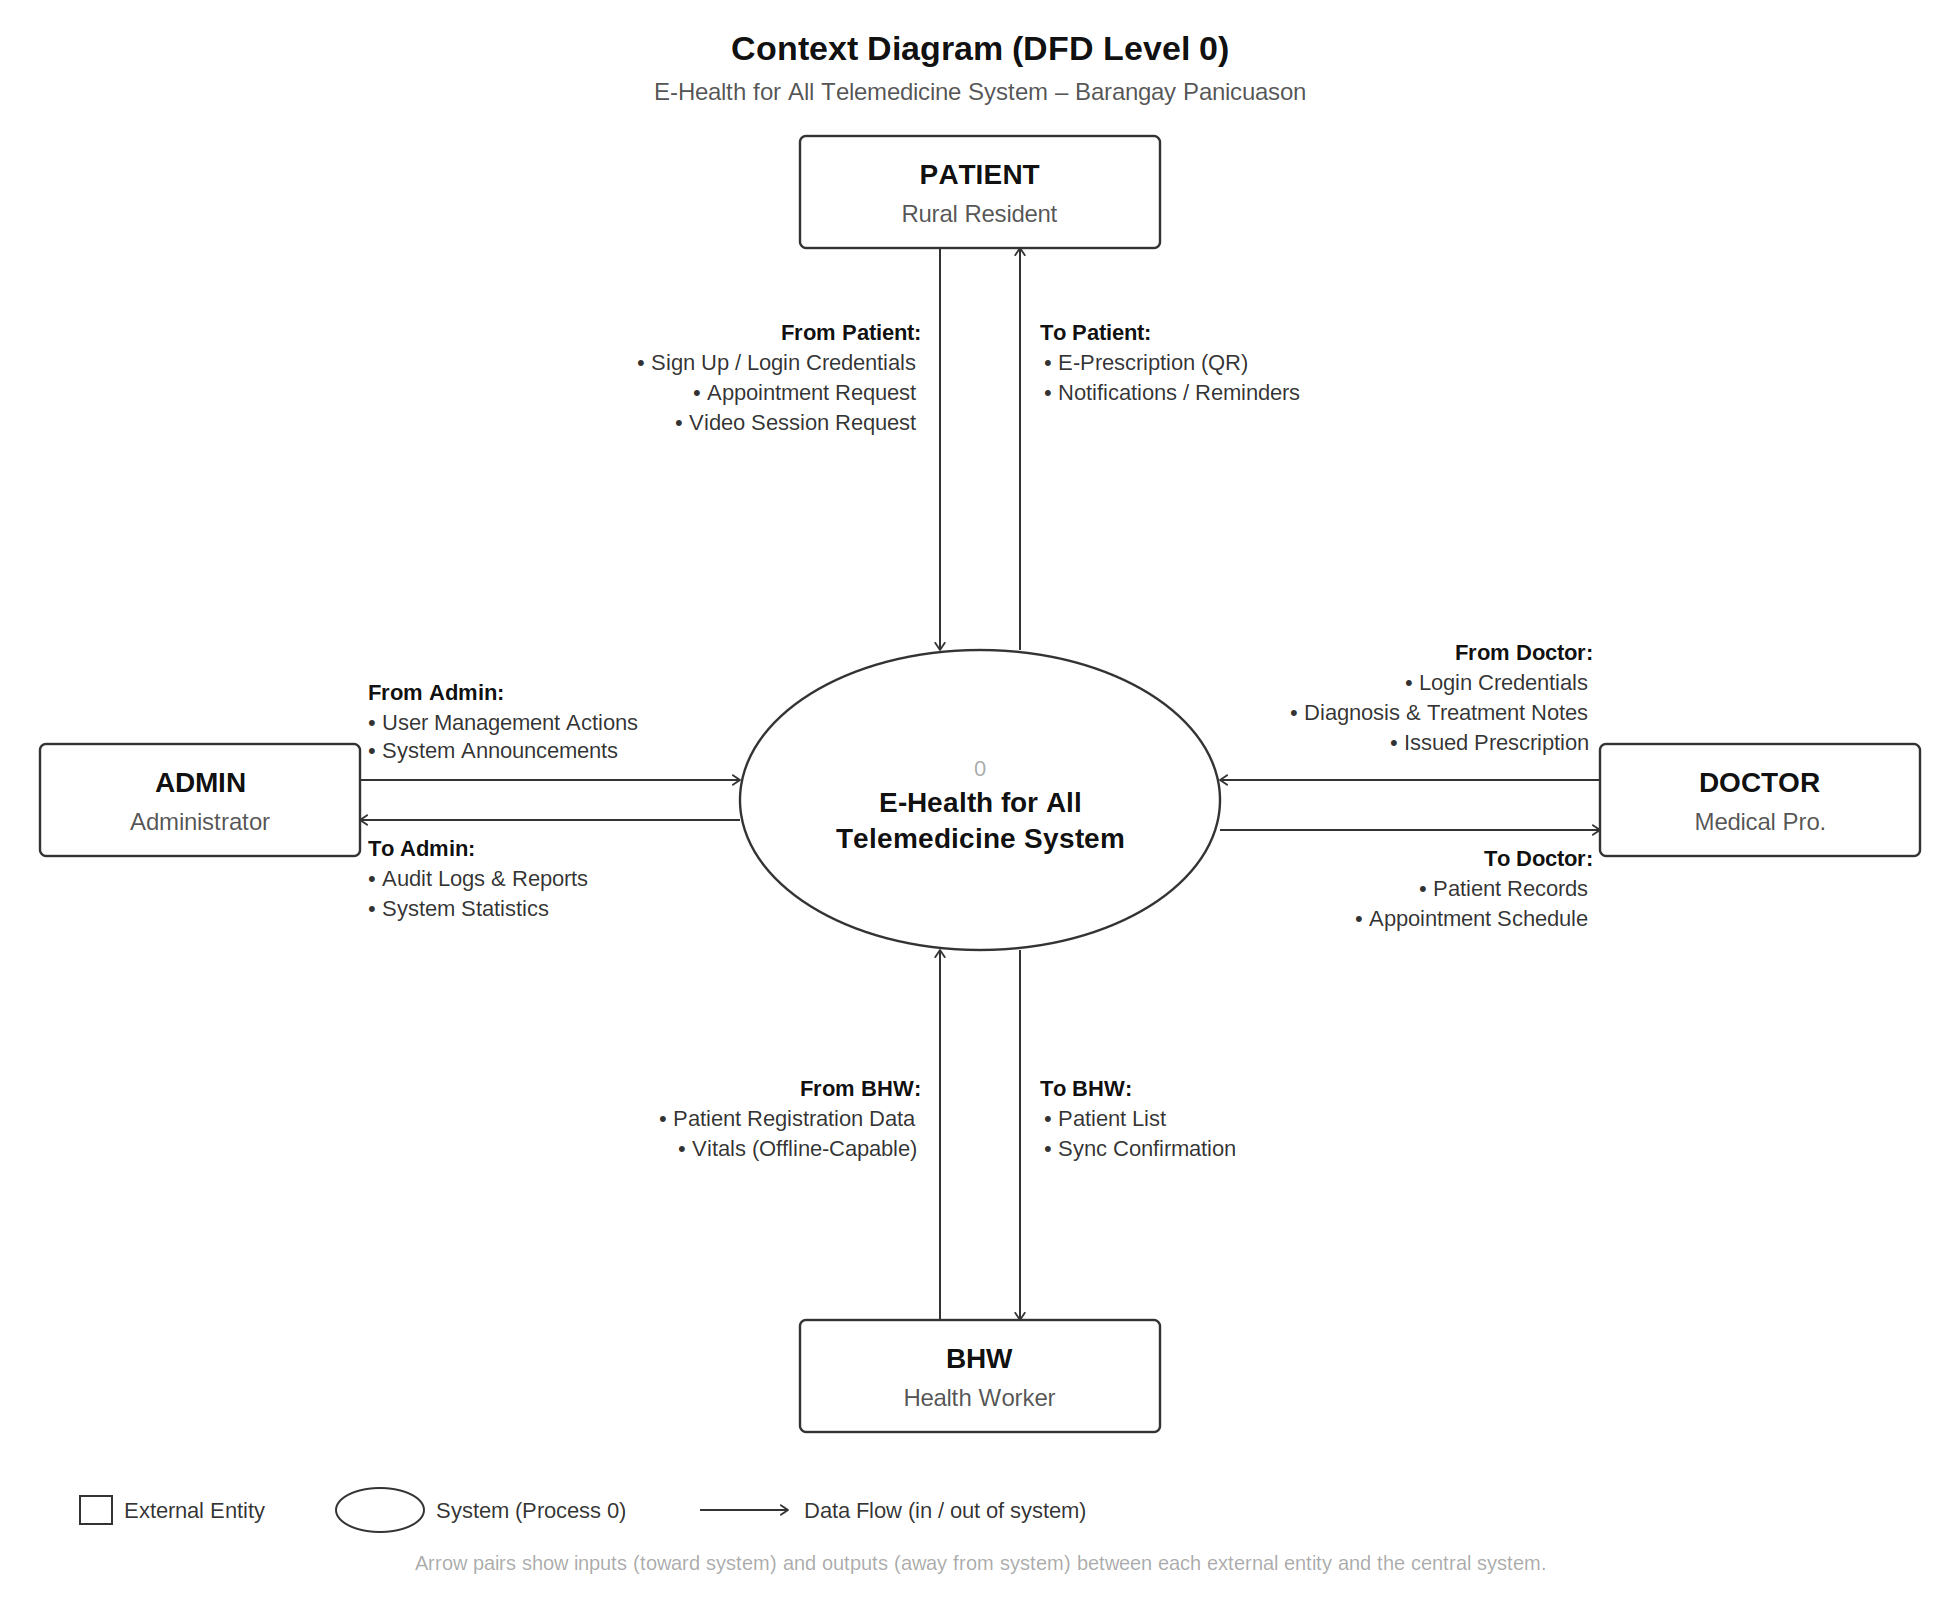
\includegraphics[width=0.95\textwidth]{dfd_level0}
    \caption{DFD Level 0}
    \label{fig:dfd_level0}
\end{figure}

\subsubsection{DFD Level 1}

The DFD Level 1 data flow diagram further breaks down the system into its main functions. For now we're comprising eight major processes that Health Connect features on its web and mobile platforms, which included Registration \& Authentication, Appointment Management, Video Consultation, Medical Record Management, e-Prescription, Vitals Management, Notification Management, and Audit \& Security. The processes outline the movement of information among the various external entities and databases.

\begin{figure}[H]
    \centering
    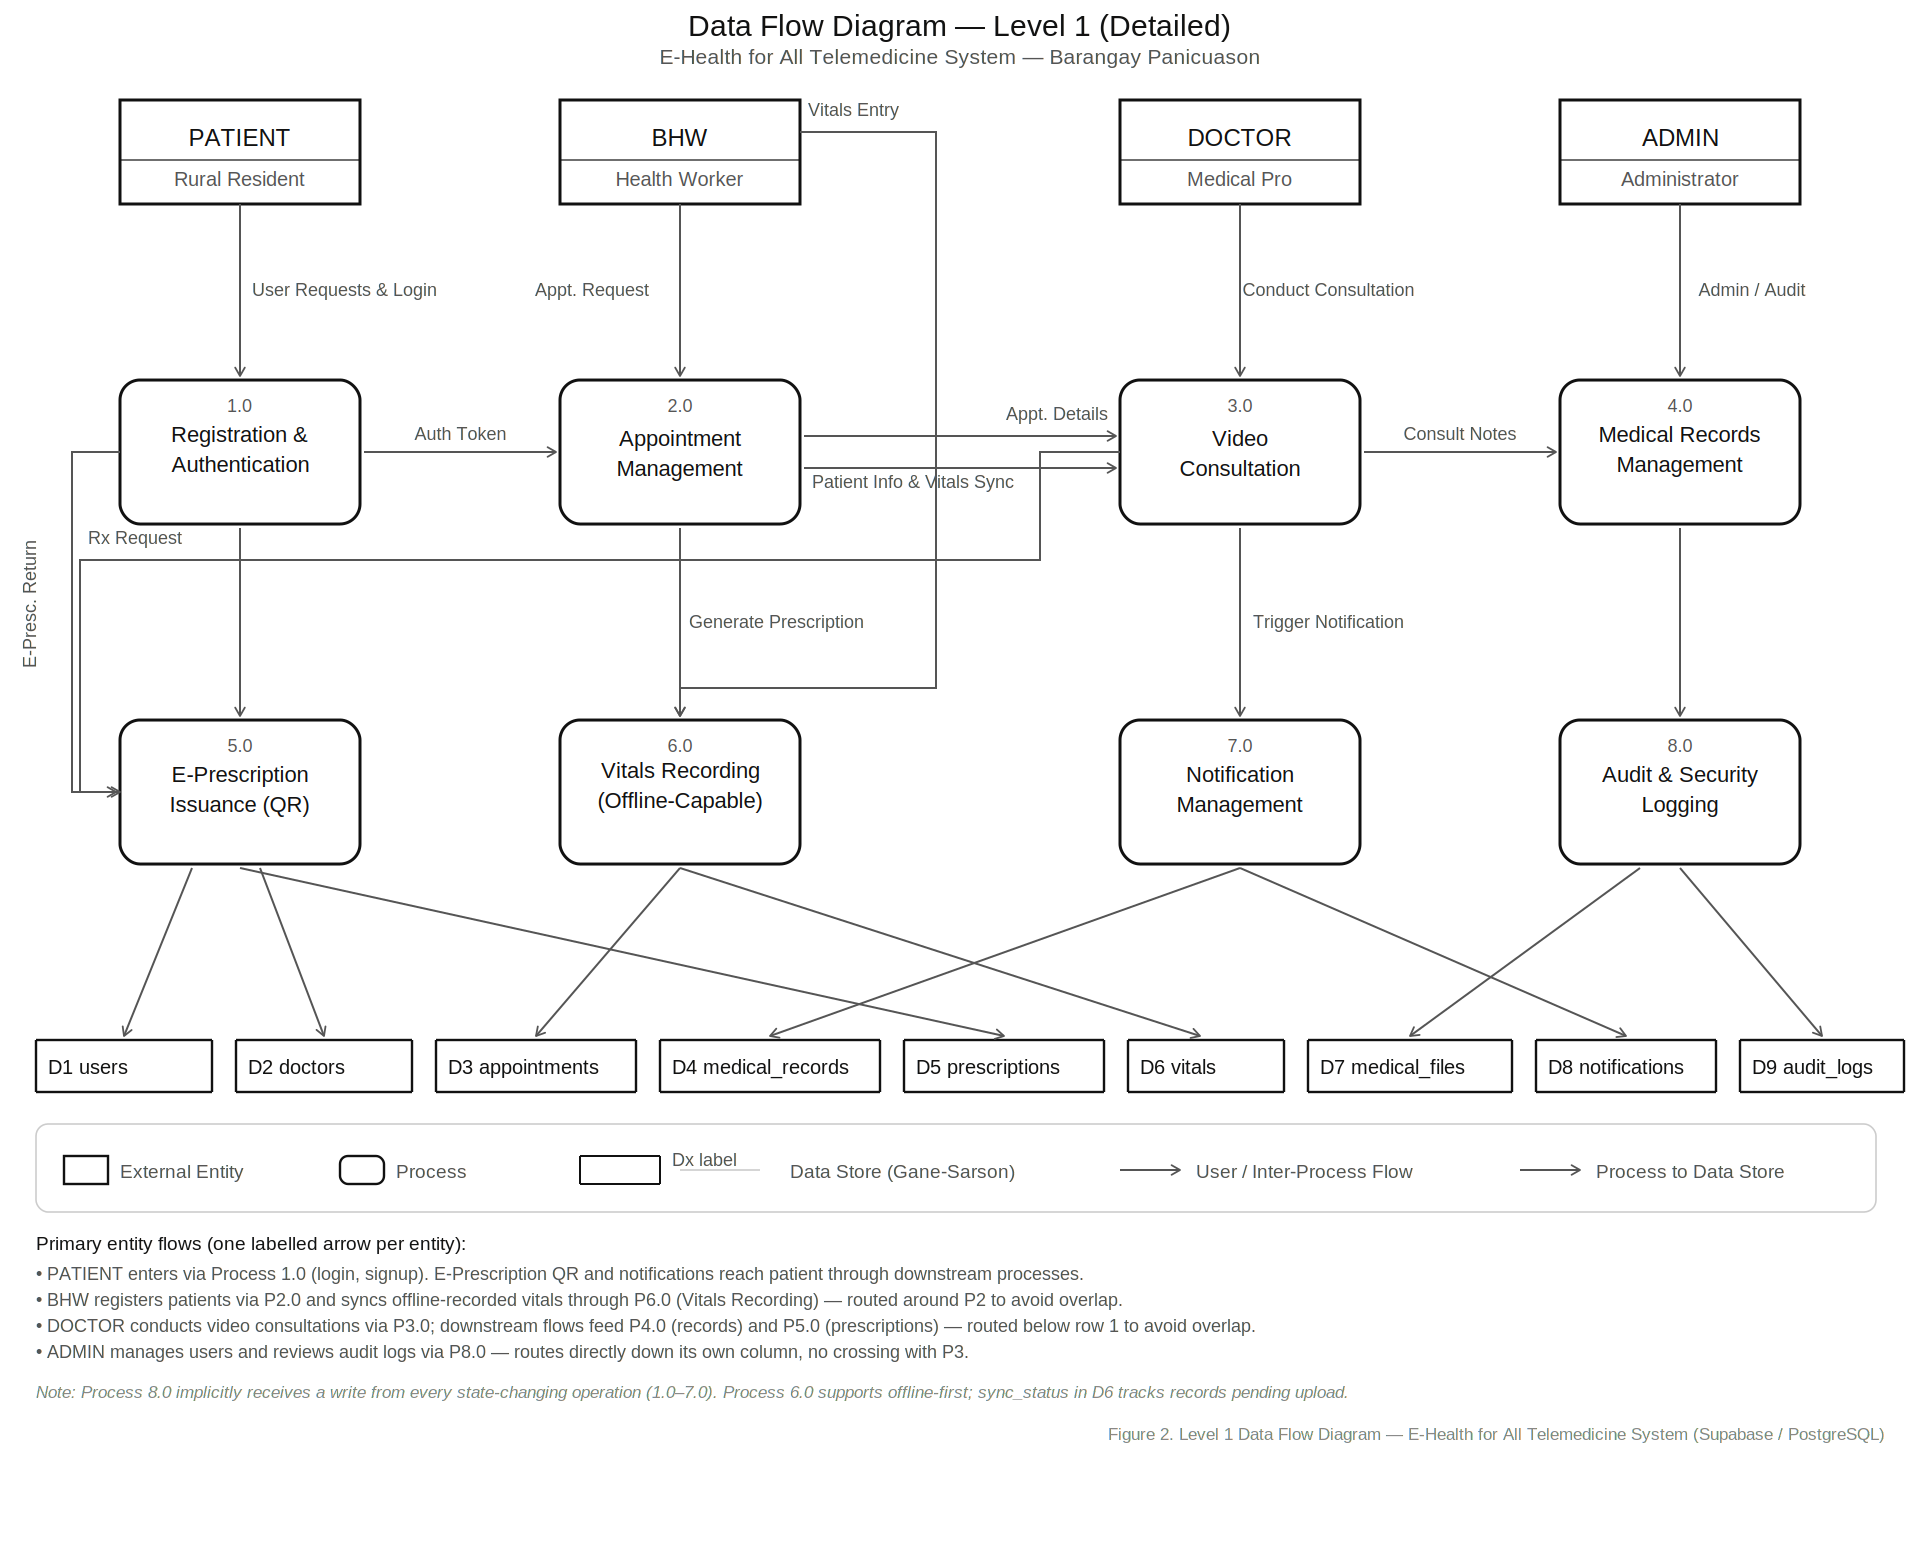
\includegraphics[width=0.95\textwidth]{dfd_level1_fixed}
    \caption{DFD Level 1}
    \label{fig:dfd_level1}
\end{figure}

% \section{Software Development Process}

\subsubsection{Entity Relationship Diagram}

The ERD visualizes each entity within the database design of the system, which is characterized by nine (9) entities, namely Users, Doctors, Appointments, Medical Records, Prescriptions, Vitals, Notifications, Audit Logs, and Medical Files. It further shows how these entities are linked through their relationships and foreign keys, thus representing the logical arrangement of the database within the system.

\begin{figure}[H]
    \centering
    \includegraphics[width=0.95\textwidth]{User-DrivenHealthcare}
    \caption{Entity Relationship Diagram}
    \label{fig:erd}
\end{figure}

\subsubsection{Data Schema}
The Data Schema presents the complete database structure of the E-Health for All Telemedicine System, detailing the tables, fields, data types, and constraints that define how data is stored and managed within the system. It complements the ERD by providing a more technical view of the database design, showing the specific attributes and relationships that support the system's core functionalities.

\begin{figure}[H]
    \centering
    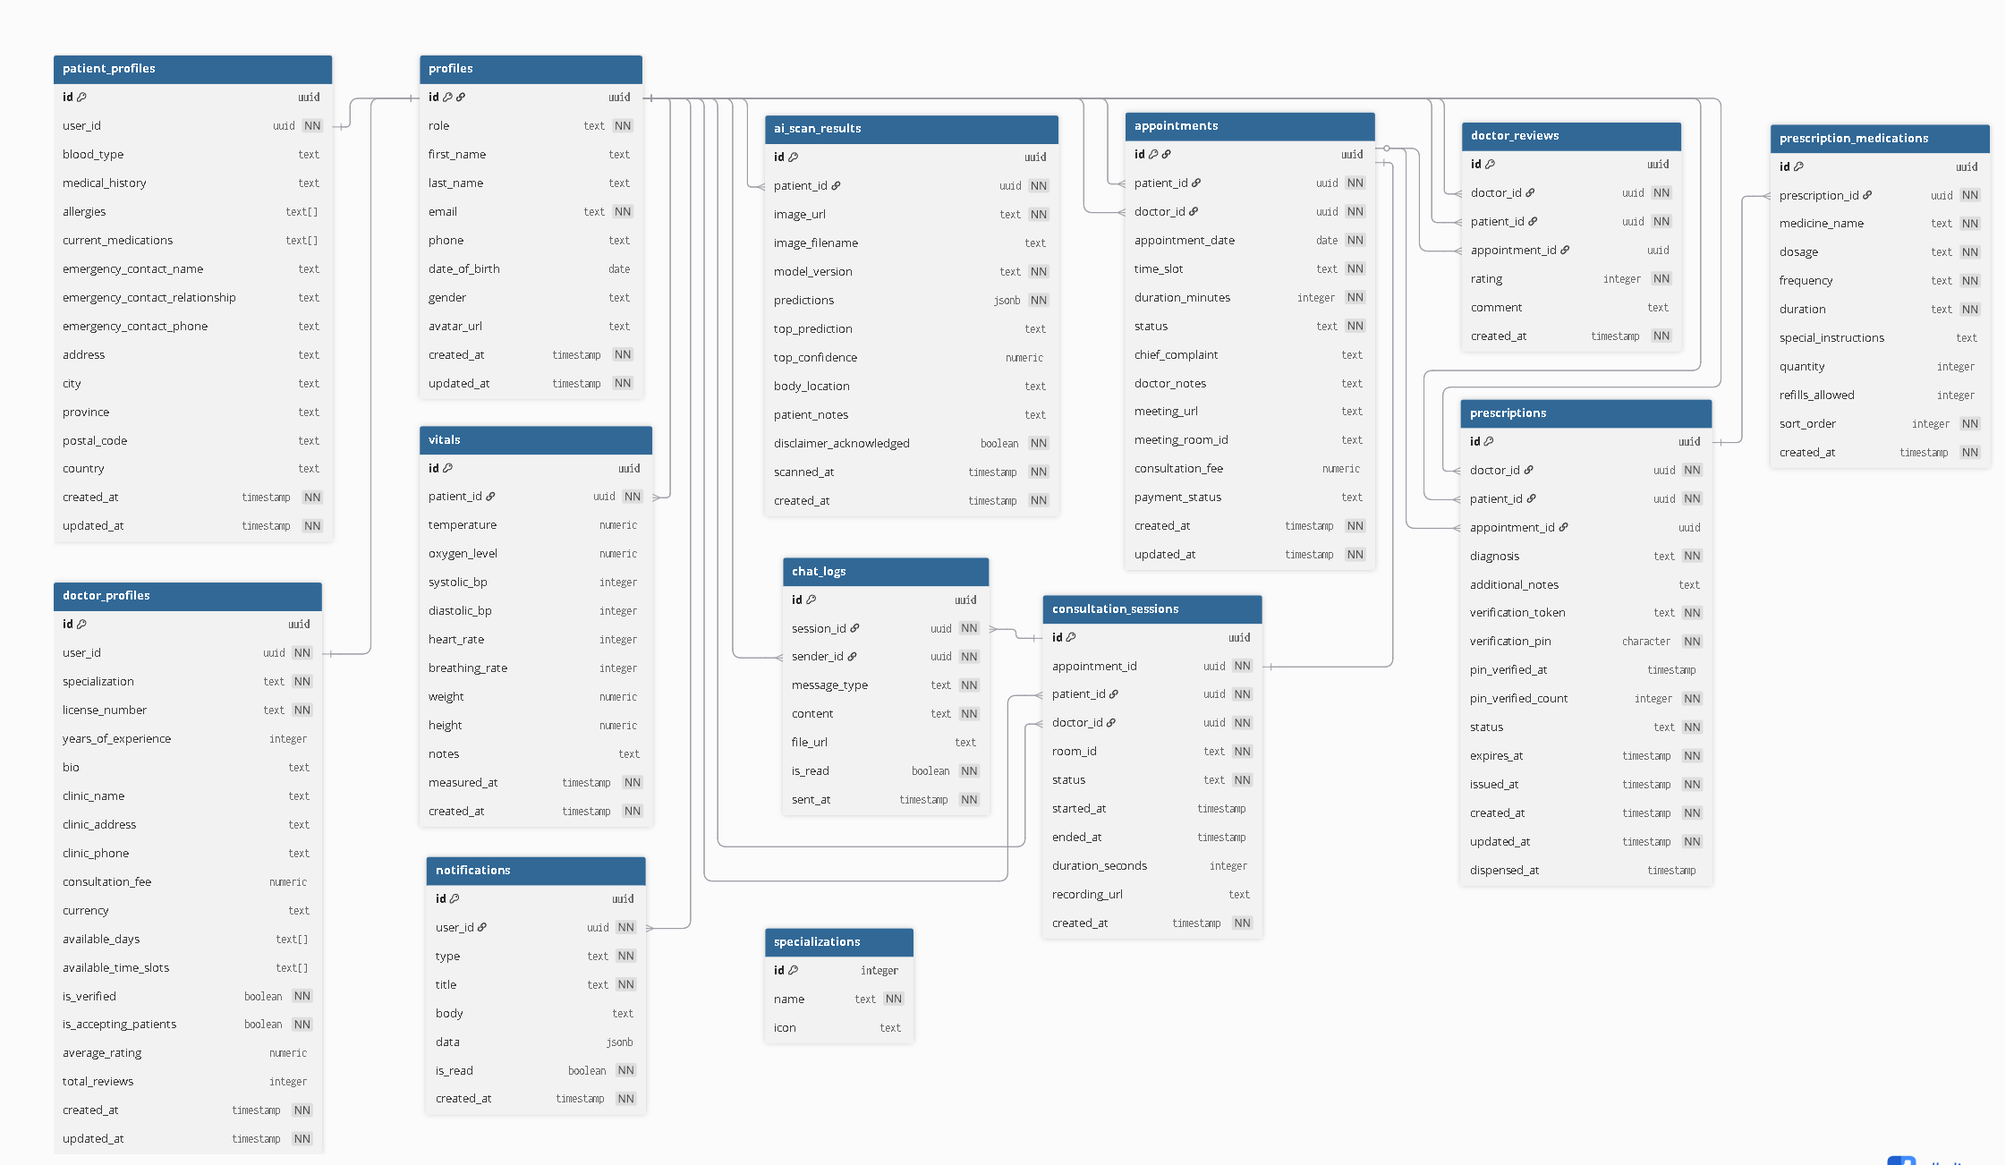
\includegraphics[width=0.95\textwidth]{data schema}
    \caption{Data Schema}
    \label{fig:dataschema}
\end{figure}

\subsection{System Architecture}	

\indent The E-Health for All Telemedicine System architecture, shown in Figure 5, connects three stakeholder groups healthcare providers, rural residents, and system administrators through a layered structure spanning user devices, connectivity, application services, integration, and data storage. The system is built around three core components in the Application Layer: (1) a web-based platform for healthcare providers, offering secure login, patient records management, clinical documentation, and digital prescription and certificate generation; (2) a mobile application for rural residents, enabling appointment scheduling, medical record access, video consultations, SMS reminders, health education content, and emergency contacts; and (3) a doctor and health worker scheduling system, maintaining provider profiles including specializations, availability, and consultation details 

\begin{figure}[H]
    \centering
    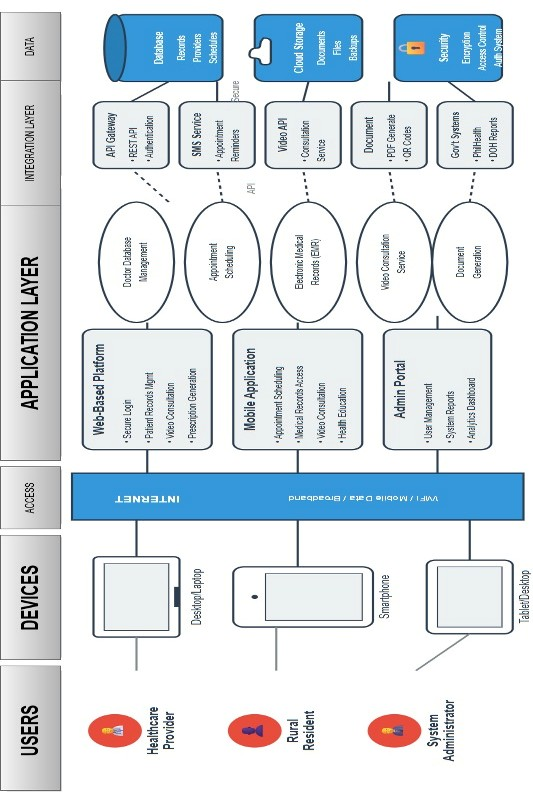
\includegraphics[width=0.95\textwidth]{E-Health_for_All_System_design_Architecture}
    \caption {System Design Architecture of E-Health for All System}
    \label{fig:architecture}
\end{figure}

% \subsection{Data Flow Diagrams}

\section{Validation and Testing Methods}

To ensure the comprehensive validation and testing of the system's quality and reliability, multiple testing methodologies were employed throughout the development process.

\textbf{Functionality Testing.} Unit testing verified individual components using test cases covering normal inputs, edge cases, and invalid inputs. Integration testing confirmed that data flowed correctly between modules and that integrated components worked together as expected. This approach ensured that each system component functioned correctly both independently and as part of the integrated system.

\textbf{User Acceptance Testing.} This involved healthcare providers evaluating whether the system met their needs through a structured checklist validating that all functional requirements were implemented. Healthcare workers and administrators participated in real-world scenario testing to verify that the system addressed their operational needs and workflow requirements.

\textbf{Performance Testing.} Load testing simulated 10, 20, and 30 concurrent users to ensure acceptable performance under typical and peak loads. Response time was tracked with a target of under 3 seconds for most operations, ensuring a smooth user experience. Offline functionality testing confirmed data entry and retrieval capabilities without internet connection, which is critical for rural healthcare settings with intermittent connectivity.

\textbf{Security Testing.} Access control verification confirmed users could only access role-appropriate features and that unauthorized access attempts were blocked. Data encryption validation confirmed sensitive information was encrypted in transit via HTTPS and at rest in the database. Passwords were hashed using strong algorithms, and sessions were tested for appropriate expiration and hijacking prevention to protect patient confidentiality and data integrity.

\textbf{Usability Testing.} The think-aloud protocol was conducted with 5 to 8 representative users who verbalized their thoughts while completing tasks as researchers observed and recorded difficulties and errors. Metrics included task completion rates, time on-task, error rates, and post-task satisfaction ratings. This qualitative and quantitative approach provided insights into user experience and identified areas for interface improvement.


\clearpage

%-----------------------------
% Chapter 3
%-----------------------------
\chapter{Results and Discussions}
This chapter presents the findings gathered from the survey administered to the health facility personnel and the barangay residents of Barangay Panicuason Rural Health Unit in Naga City. Results are organized according to the specific research objectives: (1) current healthcare practices, (2) challenges encountered in the current system, (3) system design plans as the prototype response to identified challenges, and (4) the level of acceptability of the initial prototype in terms of usability, reliability, and data security. Data are presented using weighted mean scores and frequency distributions, discussed in relation to the reviewed literature, and linked to the theoretical frameworks guiding the study. 

\section{Profile of Respondents}
A total of 93 respondents completed the survey questionnaire during the data-gathering phase. Table 3.1 presents the demographic profile. 

The respondents were predominantly of rural resident-users (86.02\%), with health facility personnel comprising the remaining 13.98\% consistent with the study's aim to prioritize the perspective of the system's primary end-users while still capturing the operational viewpoint of healthcare providers. The respondents were predominantly female (58.06\%), reflecting both the largely female composition of the community health workforce in Panicuason and the higher representation of women among surveyed residents. The majority fell within the 35--44 age bracket (41.94\%), followed by the 25--34 bracket (26.88\%), indicating a relatively young to middle-aged population that may be more receptive to adopting digital health technologies.
 
In terms of healthcare-seeking behavior, most respondents visited the RHU 4--6 times (36.56\%) or 2--3 times (35.48\%) within the month, suggesting regular engagement with the facility rather than occasional or emergency-only use. Regarding digital readiness, over half of the respondents (51.61\%) reported owning a smartphone with mobile data, while 39.78\% relied on Wi-Fi or shared data access, and only 8.60\% had no personal smartphone indicating that the majority of the sampled population already possesses some level of mobile connectivity, a favorable condition for the proposed system's adoption. Travel time to the RHU was most commonly 15--30 minutes (41.94\%), with a further 17.20\% traveling more than an hour, underscoring that access barriers remain a relevant concern for a meaningful portion of the population the system is intended to serve.

These demographics align with the Task--Technology Fit (TTF) theory's premise that technology adoption is influenced by users' familiarity with and access to the tools required to perform relevant tasks \cite{ref42} in this case, the relatively high existing smartphone and data access among respondents suggests a favorable fit between the target population and a mobile-based telemedicine solution.
\begin{table}[H]
    \centering
    \caption{Demographic Profile of Survey Respondents}
    \label{tab:demographic_profile}
    \begin{tabular}{lcc}
        \toprule
        \textbf{Category} & \textbf{Frequency (f)} & \textbf{Percentage (\%)} \\
        \midrule
        
        % RESPONDENT TYPE
        \multicolumn{3}{l}{\textbf{Respondent Type}} \\
        \hspace{1em} Health Facility & 13 & 13.98\% \\
        \hspace{1em} Resident        & 80 & 86.02\% \\
        \hspace{1em} \textbf{Total}  & \textbf{93} & \textbf{100\%} \\
        \addlinespace
        
        % SECTION A
        \multicolumn{3}{l}{\textbf{A. Sex}} \\
        \hspace{1em} Female & 54 & 58.06\% \\
        \hspace{1em} Male   & 39 & 41.94\% \\
        \hspace{1em} \textbf{Total} & \textbf{93} & \textbf{100\%} \\
        \addlinespace
        
        % SECTION B
        \multicolumn{3}{l}{\textbf{B. Age Bracket}} \\
        \hspace{1em} Below 25 years old      & 10 & 10.75\% \\
        \hspace{1em} 25 -- 34 years old      & 25 & 26.88\% \\
        \hspace{1em} 35 -- 44 years old      & 39 & 41.94\% \\
        \hspace{1em} 45 -- 59 years old      & 17 & 18.28\% \\
        \hspace{1em} 65 years old and above  & 2  & 2.15\%  \\
        \hspace{1em} \textbf{Total}          & \textbf{93} & \textbf{100\%} \\
        \addlinespace
        
        % SECTION C
        \multicolumn{3}{l}{\textbf{C. Frequency of Visits to Brgy. Panicuason RHU}} \\
        \hspace{1em} Once at a time     & 11 & 11.83\% \\
        \hspace{1em} 2 -- 3 times       & 33 & 35.48\% \\
        \hspace{1em} 4 -- 6 times       & 34 & 36.56\% \\
        \hspace{1em} More than 6 times  & 15 & 16.13\% \\
        \hspace{1em} \textbf{Total}     & \textbf{93} & \textbf{100\%} \\
        \addlinespace
        
        % SECTION D
        \multicolumn{3}{l}{\textbf{D. Access to Mobile Data and Internet}} \\
        \hspace{1em} Yes, I own a smartphone with mobile data & 48 & 51.61\% \\
        \hspace{1em} Yes, but I rely on Wi-Fi/shared data      & 37 & 39.78\% \\
        \hspace{1em} No personal smartphone                   & 8  & 8.60\%  \\
        \hspace{1em} \textbf{Total}                           & \textbf{93} & \textbf{100\%} \\
        \addlinespace
        
        % SECTION E
        \multicolumn{3}{l}{\textbf{E. Travel Time to RHU}} \\
        \hspace{1em} Less than 15 mins  & 25 & 26.88\% \\
        \hspace{1em} 15 -- 30 mins      & 39 & 41.94\% \\
        \hspace{1em} 30 -- 60 mins      & 13 & 13.98\% \\
        \hspace{1em} More than 1 hour   & 16 & 17.20\% \\
        \hspace{1em} \textbf{Total}     & \textbf{93} & \textbf{100\%} \\
        
        \bottomrule
    \end{tabular}
\end{table}

% The respondents were predominantly female (92.3\%), consistent with the largely female composition of community health workforces in Panicuason. The majority were aged 35--44 (46.2\%), indicating a relatively young and potentially technology-receptive group. In terms of work experience, most respondents had 10 years or more of service (61.54\%), followed by those with 4--6 years (30.77\%), while only a small proportion had 1--3 years (7.69\%) and none fell within the 7--9 year range. This suggests that the respondents generally possess substantial professional experience, enabling them to provide informed and reliable assessments of current operational practices. These demographics align with the Task--Technology Fit (TTF) theory's premise that technology adoption is influenced by users' experiential familiarity with their work tasks \cite{ref53}.

\newpage
\subsection{Current Practices of Rural Healthcare Providers}

\indent Research Question 1 asked: ``What are the current practices of rural healthcare providers with respect to patient records management, doctor and health worker scheduling, and appointment systems?'' Table 3.2 presents the weighted mean scores for each indicator.
With both healthcare providers and rural resident-users now represented in the sample (n=93), the results show a markedly different pattern from the facility-only findings reported previously. Patient records management remains the strongest domain (WM = 3.43, Often), but the overall rating dropped from the earlier ``Always'' (WM = 4.60) to ``Often,'' driven largely by resident perceptions of their own access to records (Item 2.5, WM = 2.92, Sometimes) a dimension the facility-only survey never captured, since staff were only assessing their own internal documentation practices, not what patients experience on the receiving end.

Doctor scheduling and appointment systems both declined to ``Sometimes'' (WM = 3.02 and 2.93, respectively), compared to ``Often'' in the facility-only round. This gap suggests that while staff perceive their own scheduling and booking processes as reasonably functional, residents do not experience the same level of reliability from their side of the interaction they are less confident that appointments are booked conveniently (Item 2.15, WM = 2.98) or that availability is known to them in advance (Item 2.7, WM = 3.08).

This divergence between provider self-assessment and patient-facing experience is consistent with [CITATION NEEDED --- provider-patient perception gap literature], and reinforces the Task--Technology Fit \cite{ref55} rationale for the proposed system: a digital platform must not only support staff workflows but close the visibility gap that residents currently experience regarding their own records, worker availability, and appointment status.

\begin{table}[H]
\centering
\footnotesize\textit{Scale: 5 = Always (4.21--5.00), 4 = Often (3.41--4.20), 3 = Sometimes (2.61--3.40), 2 = Rarely (1.81--2.60), 1 = Never (1.00--1.80)}
\label{tab:current_practices}
\renewcommand{\arraystretch}{1.1}
\begin{tabular}{>{\raggedright\arraybackslash}p{9cm} c c}
\toprule
\textbf{Indicator} & \textbf{WM} & \textbf{Interpretation} \\
\midrule

\multicolumn{3}{l}{\textbf{A. Patient Records Management}} \\
\quad 2.1 Records documented immediately after each consultation             & 3.86 & Often \\
\quad 2.2 Records stored in an organized and accessible manner               & 3.31 & Sometimes \\
\quad 2.3 Records updated regularly to reflect current health status         & 3.38 & Sometimes \\
\quad 2.4 Records retrieved quickly and accurately when needed               & 3.69 & Often \\
\quad 2.5 Patients able to view, access, or receive a copy of their records  & 2.92 & Sometimes \\
\quad \textbf{Overall Weighted Mean --- Patient Records Management}          & \textbf{3.43} & \textbf{Often} \\
\midrule

\multicolumn{3}{l}{\textbf{B. Doctor and Health Worker Scheduling}} \\
\quad 2.6 Schedules planned and communicated in advance                       & 3.11 & Sometimes \\
\quad 2.7 Availability clearly recorded and accessible to staff               & 3.08 & Sometimes \\
\quad 2.8 Schedule changes updated and communicated promptly                  & 3.17 & Sometimes \\
\quad 2.9 Backup/replacement arranged when scheduled worker is unavailable    & 3.31 & Sometimes \\
\quad 2.10 Schedules managed to minimize conflicts/overlaps                   & 3.42 & Often \\
\quad \textbf{Overall Weighted Mean --- Doctor Scheduling}                    & \textbf{3.02} & \textbf{Sometimes} \\
\midrule

\multicolumn{3}{l}{\textbf{C. Appointment Systems}} \\
\quad 2.11 Appointments arranged in an orderly and systematic manner          & 4.50 & Sometimes \\
\quad 2.12 Patients informed of appointment schedules in advance             & 4.50 & Sometimes \\
\quad 2.13 Appointment records maintained accurately to avoid double-booking  & 4.30 & Sometimes \\
\quad 2.14 Patients attended within a reasonable waiting time                 & 2.98 & Sometimes \\
\quad 2.15 Appointments can be booked/confirmed conveniently                  & 4.20 & Sometimes \\
\quad \textbf{Overall Weighted Mean --- Appointment Systems}                  & \textbf{3.03} & \textbf{Sometimes} \\
\bottomrule
\end{tabular}

\vspace{4pt}
\caption{Current Practices of Rural Healthcare Providers}
\end{table}

% Scheduling challenges averaged 3.26 (Sometimes overall), with the lack of a clear or updated availability record including uncommunicated changes scoring highest at 3.62 (Often), followed closely by health workers being assigned to multiple duties simultaneously at 3.72 (Often). This aligns with Mendoza, Cruz, and Santos \cite{ref28}, who found that the absence of a centralized scheduling system in Philippine rural health units contributes to coordination failures, particularly during peak consultation periods. Appointment system challenges averaged 3.58 (Often) the most severe domain in the combined results with the absence of an organized tracking system (WM = 3.73) and double-bookings or missed appointments without notice (WM = 3.69) as the most persistent issues. Del Rosario \cite{ref50} similarly found that the lack of digital appointment management in Philippine rural health centers contributes significantly to extended waiting times and patient dissatisfaction, a pattern reflected here in the elevated rating for long waiting times before being attended to (WM = 3.40).

% These elevated ratings higher than the facility-only round, where the same domains averaged only ``Sometimes'' indicate that rural resident-users experience appointment-related breakdowns more acutely than facility staff report experiencing them from their own operational vantage point. This gap between provider self-assessment and patient-facing experience reinforces that the challenges are not merely occasional lapses but a recurring pattern of inefficiency that compounds over time, particularly in the appointment and scheduling domains. These findings validate the need for a digital solution that addresses record organization, scheduling conflict detection, appointment tracking, and automated reminders all of which are core features of the proposed E-Health for All system.
\subsection{Challenges Encountered in the Current System}

\indent Research Question 2 asked: ``What are the challenges encountered in the current system?'' Table 3.3 presents the weighted mean scores for each challenge indicator. All challenge indicators were rated in the ``Sometimes'' range (WM = 3.25--3.40), confirming that while problems were not constant, they occurred with enough regularity to warrant systematic intervention. The most frequently cited challenge across domains was the difficulty in organizing and managing patient records (WM = 3.29), consistent with findings by D'Amore et al. \cite{ref12} that paper-based record systems in rural health facilities are particularly susceptible to organizational lapses due to high patient volumes and limited administrative staffing.

\begin{table}[H]
\centering
\footnotesize\textit{Scale: 5 = Always (4.21--5.00), 4 = Often (3.41--4.20), 3 = Sometimes (2.61--3.40), 2 = Rarely (1.81--2.60), 1 = Never (1.00--1.80)}
\label{tab:challenges}
\renewcommand{\arraystretch}{1.1}
\begin{tabular}{>{\raggedright\arraybackslash}p{9cm} c c}
\toprule
\textbf{Challenge Indicator} & \textbf{WM} & \textbf{Interpretation} \\
\midrule

\multicolumn{3}{l}{\textbf{A. Patient Records Management}} \\
\quad 3.1 Patient records are difficult to organize and manage                    & 3.20 & Sometimes \\
\quad 3.2 Patient records are missing or incomplete                               & 2.99 & Sometimes \\
\quad 3.3 Records are lost, damaged, or difficult to verify for accuracy          & 3.68 & Often \\
\quad 3.4 Limited information on what health data is being recorded              & 3.25 & Sometimes \\
\quad \textbf{Overall Weighted Mean --- Patient Records Challenges}               & \textbf{3.29} & \textbf{Sometimes} \\
\midrule

\multicolumn{3}{l}{\textbf{B. Doctor and Health Worker Scheduling}} \\
\quad 3.5 Scheduling conflicts among doctors/health workers occur                & 3.06 & Sometimes \\
\quad 3.6 No clear or updated record of availability                             & 3.62 & Sometimes \\
\quad 3.7 Health workers assigned to multiple duties simultaneously              & 3.72 & Often \\
\quad 3.8 Schedule changes not communicated to concerned staff                    & 2.62 & Sometimes \\
\quad \textbf{Overall Weighted Mean --- Scheduling Challenges}                    & \textbf{3.26} & \textbf{Sometimes} \\
\midrule

\multicolumn{3}{l}{\textbf{C. Appointment Systems}} \\
\quad 3.9 Patients experience long waiting times before being attended to        & 3.40 & Sometimes \\
\quad 3.10 Delays in processing patient appointments                             & 3.48 & Often \\
\quad 3.11 Double-bookings or missed appointments occur                          & 3.69 & Often \\
\quad 3.12 No organized system for tracking or confirming appointments           & 3.73 & Often \\
\quad \textbf{Overall Weighted Mean --- Appointment Challenges}                  & \textbf{3.37} & \textbf{Sometimes} \\
\bottomrule
\end{tabular}

\vspace{4pt}
\caption{Challenges in Current Healthcare Practices}
\end{table}

Scheduling challenges averaged 3.26 (Sometimes overall), with the lack of a clear or updated availability record including uncommunicated changes scoring highest at 3.62 (Often), followed closely by health workers being assigned to multiple duties simultaneously at 3.72 (Often). This aligns with Mendoza, Cruz, and Santos \cite{ref28}, who found that the absence of a centralized scheduling system in Philippine rural health units contributes to coordination failures, particularly during peak consultation periods. Appointment system challenges averaged 3.58 (Often) the most severe domain in the combined results with the absence of an organized tracking system (WM = 3.73) and double-bookings or missed appointments without notice (WM = 3.69) as the most persistent issues. Del Rosario \cite{ref50} similarly found that the lack of digital appointment management in Philippine rural health centers contributes significantly to extended waiting times and patient dissatisfaction, a pattern reflected here in the elevated rating for long waiting times before being attended to (WM = 3.40).

These elevated ratings higher than the facility-only round, where the same domains averaged only ``Sometimes'' indicate that rural resident-users experience appointment-related breakdowns more acutely than facility staff report experiencing them from their own operational vantage point. This gap between provider self-assessment and patient-facing experience reinforces that the challenges are not merely occasional lapses but a recurring pattern of inefficiency that compounds over time, particularly in the appointment and scheduling domains. These findings validate the need for a digital solution that addresses record organization, scheduling conflict detection, appointment tracking, and automated reminders all of which are core features of the proposed E-Health for All system.

% -------------------------------------------------------
\subsection{System Design and Plans for the Prototype}

\indent Research Question 3 asked: “What system can be designed to address the identified challenges?” This section presents the importance ratings for proposed system features. Table 3.4 describes the design plans for the prototype, including the use case, workflow, and database schema. 

\begin{table}[H]
\centering
\label{tab:proposed_features}
\renewcommand{\arraystretch}{1.1}
\footnotesize\textit{Scale: 5 = Very Important (4.21--5.00), 4 = Important (3.41--4.20), 3 = Moderately Important (2.61--3.40), 2 = Slightly Important (1.81--2.60), 1 = Not Important (1.00--1.80)}
\begin{tabular}{>{\raggedright\arraybackslash}p{9cm} c c}
\toprule
\textbf{Proposed System Feature} & \textbf{WM} & \textbf{Interpretation} \\
\midrule
4.1 Digital storage and easy retrieval of patient records           & 4.50 & Very Important \\
4.2 Automated doctor/worker scheduling with conflict detection      & 4.50 & Very Important \\
4.3 Online patient appointment booking                              & 4.60 & Very Important \\
4.4 Automated appointment reminders and notifications               & 4.80 & Very Important \\
4.5 Secure login and role-based access control                      & 4.90 & Very Important \\
\midrule
\textbf{Overall Weighted Mean}                                      & \textbf{4.66} & \textbf{Very Important} \\
\bottomrule
\end{tabular}

\vspace{4pt}
\caption {Importance of Proposed Features}
\end{table}

All five proposed features received ``Very Important'' ratings, with an overall weighted mean of 4.66. Secure login and role-based access control (WM = 4.90) ranked highest, reflecting a strong awareness among health workers of data privacy obligations under the Data Privacy Act of 2012. Automated reminders (WM = 4.80) ranked second, directly addressing the challenge of missed appointments (Item 3.11, WM = 2.70) and long waiting times (Item 3.9, WM = 3.00). Online appointment booking (WM = 4.60) and digital storage (WM = 4.50) also scored highly, validating the core functional design of the proposed system. These ratings are consistent with the TAM framework \cite{ref56}, where perceived usefulness as evidenced by the high importance ratings is a primary determinant of technology adoption intention.

\subsection{Perceived Acceptability of the Proposed System }

\indent Research Question 4 asked: "What is the level of acceptability of the proposed system, as perceived by healthcare providers and rural resident-users, in terms of usability, reliability, and data security?" Table 3.5 presents the weighted mean scores for each indicator. 

\begin{table}[H]
\centering
\footnotesize\textit{Scale: 5 = Completely Agree (4.21--5.00), 4 = Agree (3.41--4.20), 3 = Somewhat Agree (2.61--3.40), 2 = Slightly Agree (1.81--2.60), 1 = Not at All Agree (1.00--1.80)}
\label{tab:acceptability}
\renewcommand{\arraystretch}{1.1}
\begin{tabular}{>{\raggedright\arraybackslash}p{9cm} c c}
\toprule
\textbf{Indicator} & \textbf{WM} & \textbf{Interpretation} \\
\midrule

\multicolumn{3}{l}{\textbf{A. Usability}} \\
\quad 3.13 Easy to learn and navigate                          & 3.56 & Agree \\
\quad 3.14 Complete tasks with minimal effort                  & 3.69 & Agree \\
\quad 3.15 Instructions/prompts clear and understandable       & 3.62 & Agree \\
\quad 3.16 Design appropriate for digital skill level          & 3.01 & Somewhat Agree \\
\quad \textbf{Overall Weighted Mean --- Usability}              & \textbf{3.50} & \textbf{Agree} \\
\midrule

\multicolumn{3}{l}{\textbf{B. Reliability}} \\
\quad 3.17 Works consistently without errors/crashes           & 4.50 & Completely Agree \\
\quad 3.18 Remains usable during poor connectivity              & 3.41 & Agree \\
\quad 3.19 Available whenever needed                            & 4.03 & Agree \\
\quad 3.20 Notifications/reminders accurate and timely          & 2.33 & Slightly Agree \\
\quad \textbf{Overall Weighted Mean --- Reliability}            & \textbf{3.18} & \textbf{Somewhat Agree} \\
\midrule

\multicolumn{3}{l}{\textbf{C. Data Security}} \\
\quad 3.21 Trust system to keep health information private     & 3.05 & Somewhat Agree \\
\quad 3.22 Believe only authorized personnel can view records   & 4.21 & Completely Agree \\
\quad 3.23 Comfortable providing personal information           & 2.78 & Somewhat Agree \\
\quad 3.24 Believe system will have secure login/authentication & 4.24 & Completely Agree \\
\quad \textbf{Overall Weighted Mean --- Data Security}          & \textbf{3.53} & \textbf{Agree} \\
\bottomrule
\end{tabular}

\vspace{4pt}
\caption{Perceived Acceptability of the Proposed System}
\end{table}

The proposed system received an overall ``Agree'' rating across two of the three dimensions (Usability, WM = 3.50; Data Security, WM = 3.53), while Reliability was rated within the ``Somewhat Agree'' range (WM = 3.18), indicating a generally favorable but more cautious anticipated acceptance among respondents, particularly regarding the system's expected performance under real-world conditions.

Usability recorded the second-highest overall weighted mean (WM = 3.50, Agree). Respondents expressed the strongest confidence in their ability to complete tasks with minimal effort (Item 3.14, WM = 3.69, Agree) and in the system's ease of learning and navigation (Item 3.13, WM = 3.56, Agree). Notably, however, respondents rated the appropriateness of the system's design for their digital skill level considerably lower (Item 3.16, WM = 3.01, Somewhat Agree) --- the weakest item in this dimension. This gap between confidence in completing tasks and confidence in the design's fit for one's own digital skill level suggests that while residents anticipate the system will be functional, a segment of respondents remain uncertain whether the interface itself will accommodate varying levels of digital literacy, a concern consistent with the digital literacy barriers documented in rural Philippine telehealth literature \cite{ref6}, \cite{ref7}.

Reliability emerged as the lowest-rated and most inconsistent dimension overall (WM = 3.18, Somewhat Agree). While respondents expressed strong confidence that the system would work consistently without errors or crashes (Item 3.17, WM = 4.50, Completely Agree) and would be available whenever needed (Item 3.19, WM = 4.03, Agree), this confidence dropped sharply for two items directly tied to real-world field conditions: the system remaining usable during poor connectivity (Item 3.18, WM = 3.41, Agree, at the lower boundary of the band) and, most notably, the accuracy and timeliness of notifications and reminders (Item 3.20, WM = 2.33, Slightly Agree) --- the lowest-scoring item across the entire table. This pattern suggests that respondents distinguish between the system's core technical stability, which they view favorably, and its dependence on external factors such as internet connectivity and message delivery, which they view with considerably more skepticism. This is consistent with the connectivity and infrastructure barriers already identified in the Introduction and Gap Bridged sections as unresolved constraints in Barangay Panicuason, and reinforces that residents' skepticism is grounded in lived experience rather than unfamiliarity with the concept of telemedicine itself.

Data Security scored the highest overall (WM = 3.53, Agree), though with a similarly wide spread between items. Respondents expressed strong belief that the system would restrict record access to authorized personnel (Item 3.22, WM = 4.21, Completely Agree) and would include secure login and authentication (Item 3.24, WM = 4.24, Completely Agree). However, trust that the system would keep health information private (Item 3.21, WM = 3.05, Somewhat Agree) and comfort in providing personal information through the system (Item 3.23, WM = 2.78, Somewhat Agree) were rated notably lower. This suggests that respondents' confidence in the system's technical security mechanisms does not fully translate into personal comfort or trust --- a distinction consistent with the Technology Acceptance Model's separation of perceived usefulness from the more subjective, trust-based dimensions of adoption intention \cite{ref56}.

Taken together, these mixed results spanning ``Slightly Agree'' to ``Completely Agree'' across individual items offer a more grounded and defensible picture of anticipated acceptability than uniformly high ratings would, reflecting genuine areas of resident confidence (core functionality, access control) alongside legitimate reservations tied to infrastructure-dependent features and personal data comfort. These reservations directly inform the system's subsequent refinement, particularly around offline reliability and privacy communication, ahead of full-scale field testing.
% \chapter*{Results and Discussions}
% This section provides a concise synthesis of the study's key findings and reflects on their broader significance in advancing rural healthcare delivery through digital innovation.

% This study aimed to design and develop E-Health for All, a user-centered telemedicine platform for Barangay Panicuason Rural Health Unit in Naga City, addressing inefficiencies in patient records management, health worker scheduling, and appointment systems. Using a developmental-descriptive research design, data were gathered from 13 health facility personnel to document current practices, identify challenges, evaluate proposed system features, and assess prototype acceptability.

% The findings reveal that health facility personnel had already established strong baseline practices across all three operational domains, indicating a structured and disciplined workforce. This is significant because it confirms that the E-Health for All system enters a context where existing workflows are well-established, making adoption more likely when the platform is designed to enhance rather than replace familiar routines consistent with the Task–Technology Fit (TTF) theory.

% Despite these strong practices, recurring challenges were confirmed across all domains. Difficulties in organizing physical records, the absence of a systematic appointment tracking mechanism, and scheduling conflicts among health workers were the most consistently reported concerns. These findings collectively validate the study's core rationale that an integrated telemedicine platform is both necessary and timely for a facility of this scale and context.

% All proposed system features were rated very important, with data security, automated reminders, and online booking receiving the highest endorsements — directly corresponding to the identified challenges. This alignment confirms that the system is grounded in users' actual needs, consistent with the Technology Acceptance Model (TAM). The respondent profile, predominantly female, relatively young, and experienced, further supports readiness for a managed digital transition as affirmed by the Diffusion of Innovations (DOI) theory.

% Overall, this study demonstrates that E-Health for All is both technically feasible and operationally justified for Barangay Panicuason RHU. Beyond its immediate application, it offers a replicable framework for designing context-sensitive telemedicine solutions in similarly resource-limited settings.


% \section*{Recomendations}
% Based on the conclusions of this study, the following recommendations are directed to the key stakeholders involved in the deployment, improvement, and continued research of the E-Health for All telemedicine system.

% For the Barangay Panicuason Health Unit and the Local Government Unit. The local government unit should pursue the formal adoption and full deployment of the E-Health for All system by allocating a dedicated budget for device procurement, internet connectivity, and system maintenance. A structured onboarding program should be conducted prior to deployment to ensure a smooth transition from paper-based to digital operations.

% For System Developers and Future Development Teams. Developers should expand the system in future iterations to include laboratory result integration, pharmacy management, a patient-facing portal, and iOS compatibility. Offline functionality should be strengthened to maintain data access during internet outages, and all development must strictly uphold the Data Privacy Act of 2012 through encryption, role-based access controls, and regular security auditing.

% For Health Facility Personnel. Health workers should actively engage during the pilot phase by documenting usability issues and communicating improvement suggestions through formal feedback channels. Their sustained adoption and cooperation will be essential to the system's continuous refinement and long-term success.

% For Academic Researchers and Future Studies. Future researchers should extend this study by including community residents as secondary respondents and conducting longitudinal evaluations to assess long-term system impact. Comparative studies across multiple rural health units are recommended, and future instruments should incorporate the System Usability Scale (SUS) and Cronbach's Alpha to strengthen methodological rigor.

% For Policymakers and the Department of Health. The Department of Health should consider the E-Health for All model as a pilot reference for rural health unit digitalization nationwide. Policymakers should provide technical and financial support to local government units pursuing similar initiatives and establish interoperability standards to connect locally developed platforms with national health systems such as iHOMIS and the National Health Data Repository.


%\subsection{Problem 2}

%\subsection{Problem 3}

%\section{Design and System Plans}

%\section{Summary of Findings}

%\section{Conclusions}

%\section{Recommendations}

%-----------------------------
% References
%-----------------------------

\clearpage
\nocite{*}
\printbibliography


\clearpage

\chapter*{Appendices}

\begin{figure}[H]
    \caption*{Appendices A-1}
    \centering
    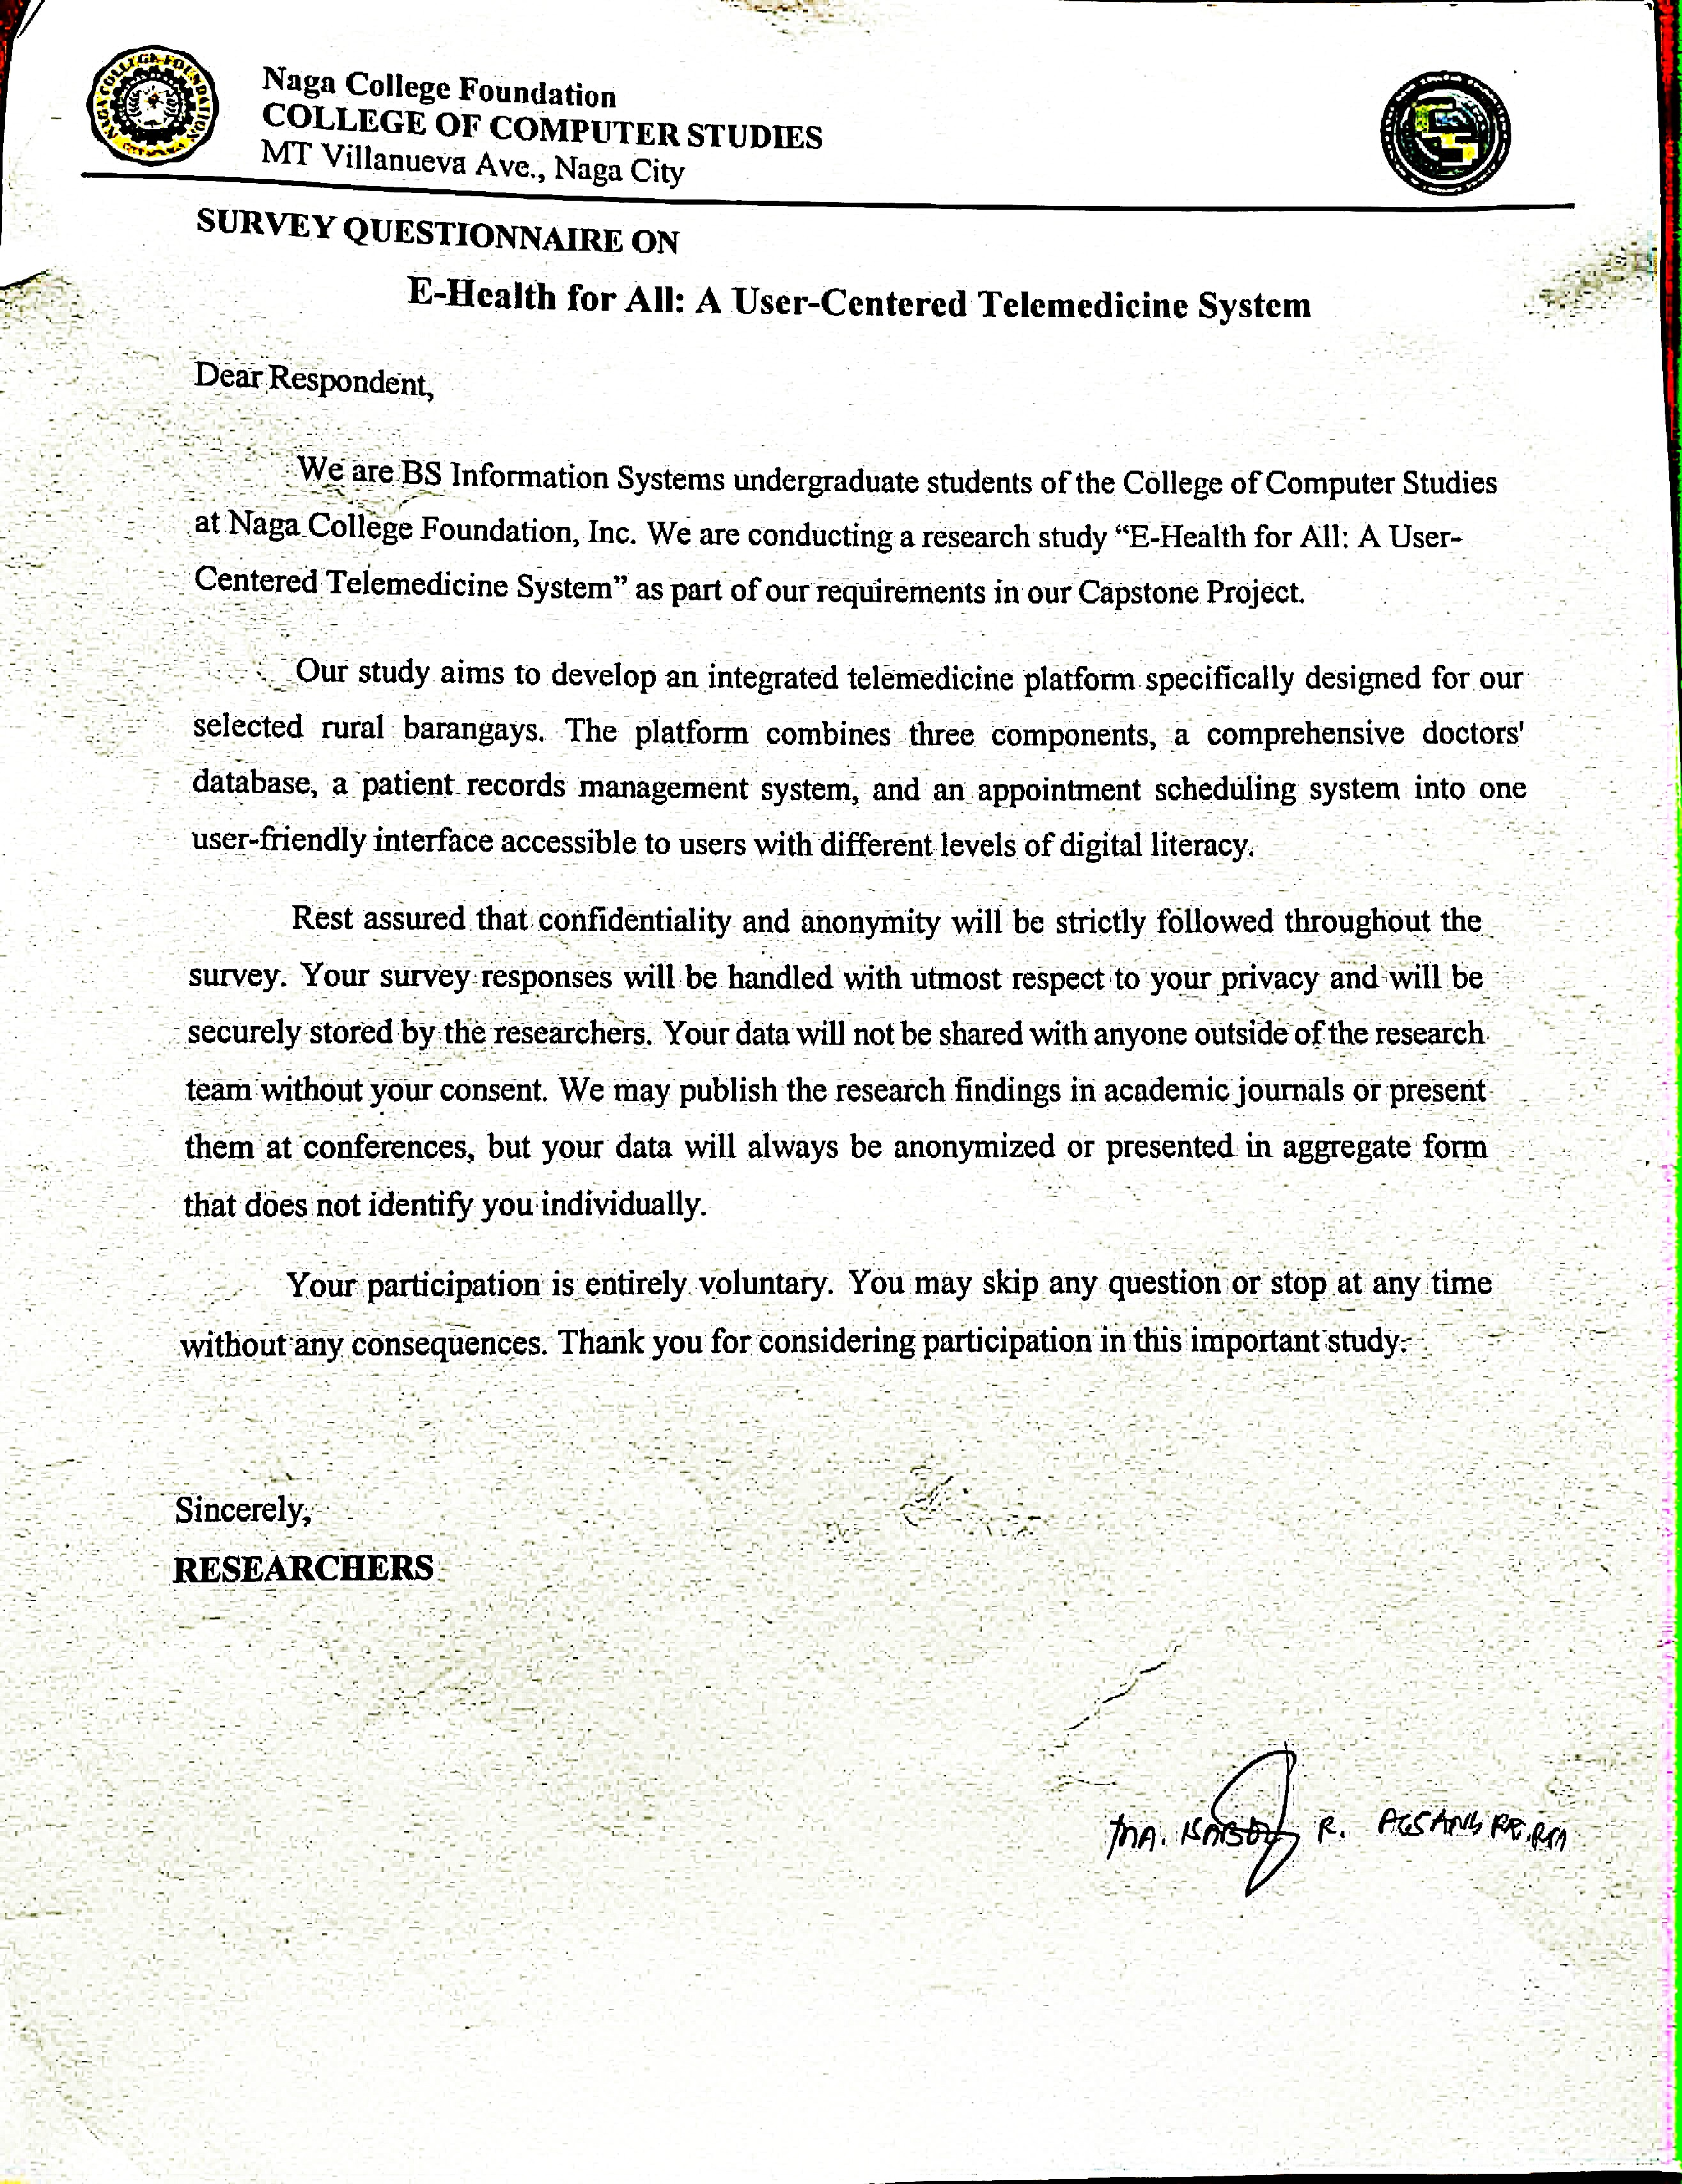
\includegraphics[width=0.95\textwidth]{1}
\end{figure}

\begin{figure}[H]
    \caption*{Appendices A-2}
    \centering
    
\includegraphics[width=0.95\textwidth]{2}
\end{figure}

\begin{figure}[H]
    \caption*{Appendices A-3}
    \centering
    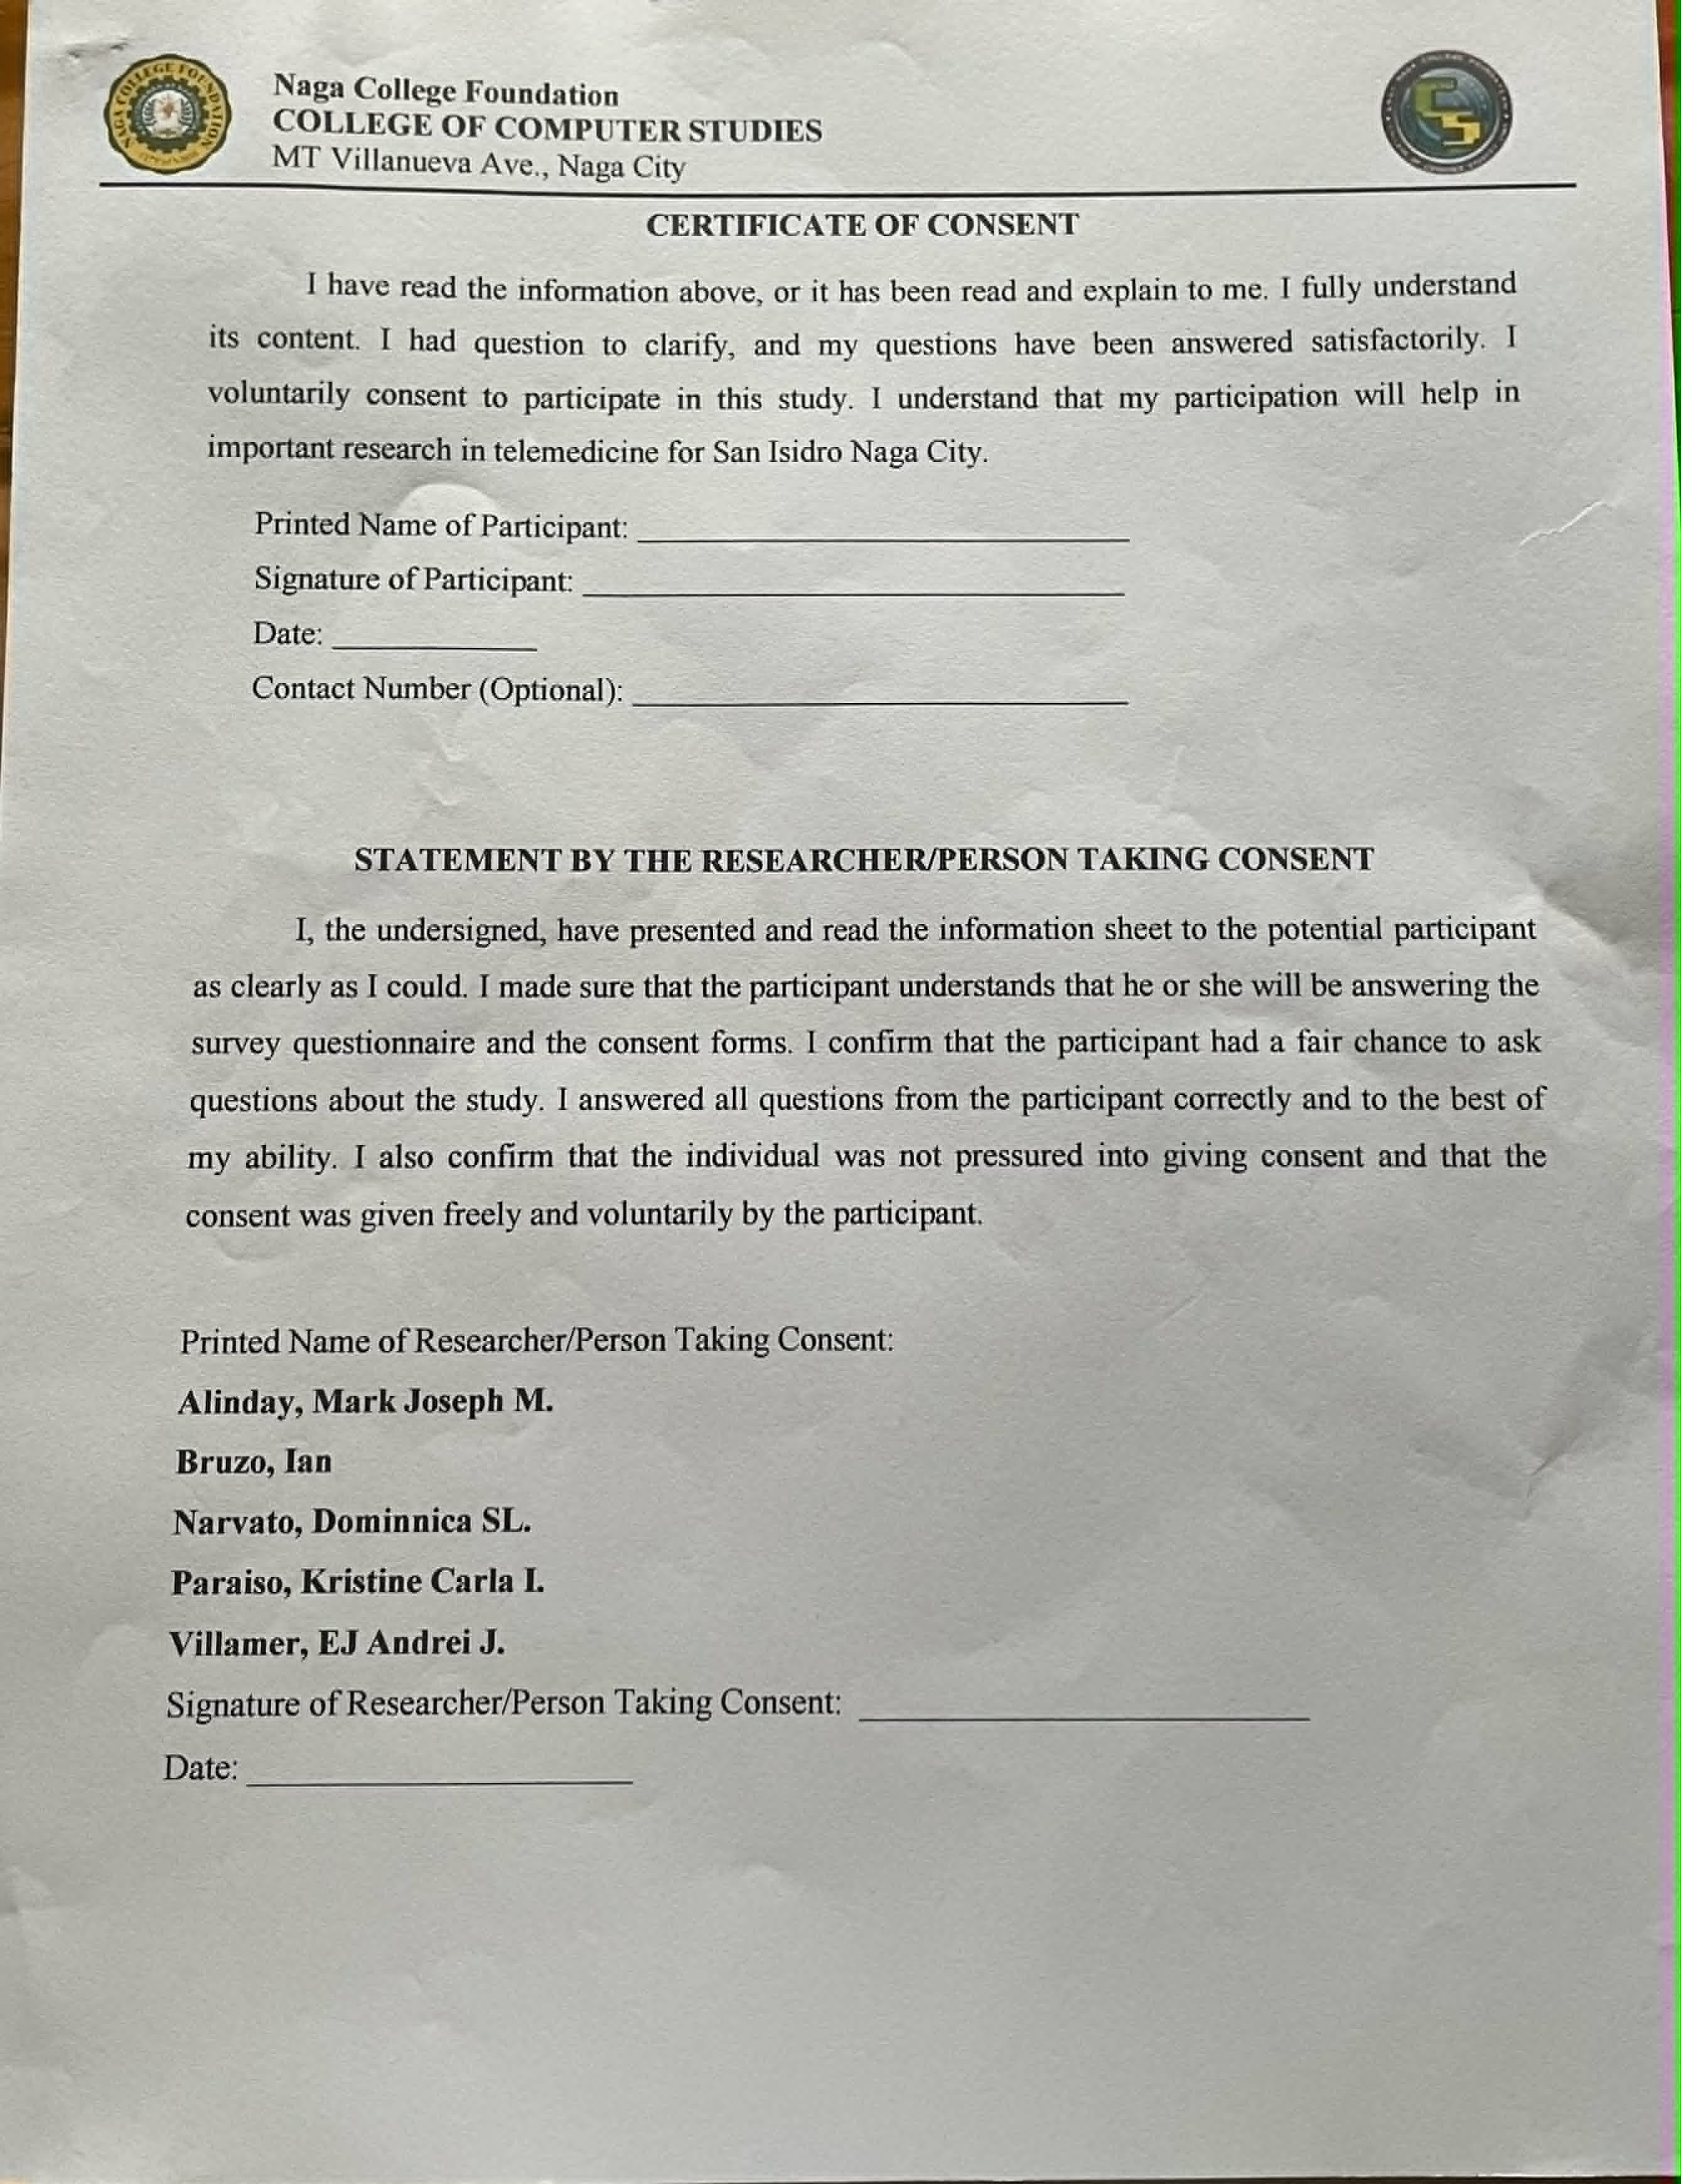
\includegraphics[width=0.95\textwidth]{3}

\end{figure}

\begin{figure}[H]
    \caption*{Appendices A-4}
    \centering
    
\includegraphics[width=0.95\textwidth]{4}
    
\end{figure}

\begin{figure}[H]
    \caption*{Appendices A-5}
    \centering
    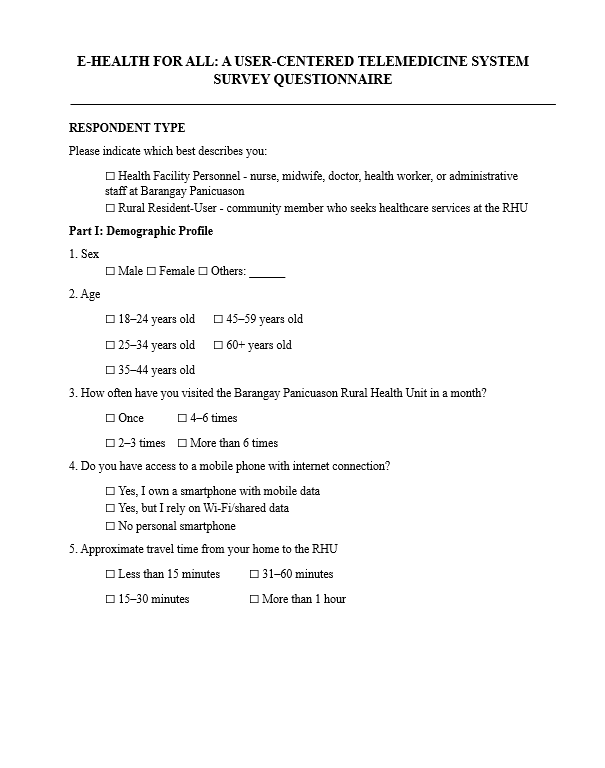
\includegraphics[width=0.95\textwidth]{1 survey(2).png}
\end{figure}

\begin{figure}[H]
    \caption*{Appendices A-6}
    \centering
    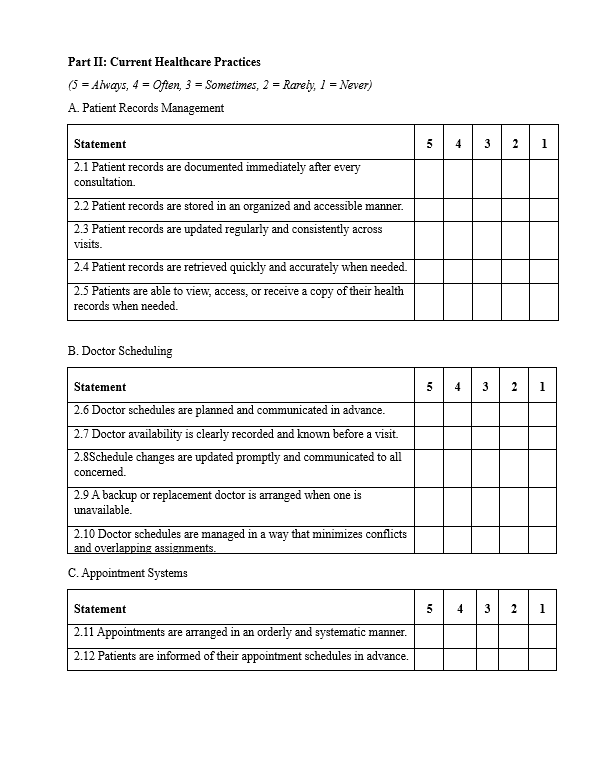
\includegraphics[width=0.95\textwidth]{2 survey(3).png}
\end{figure}

\begin{figure}[H]
    \caption*{Appendices A-7}
    \centering
    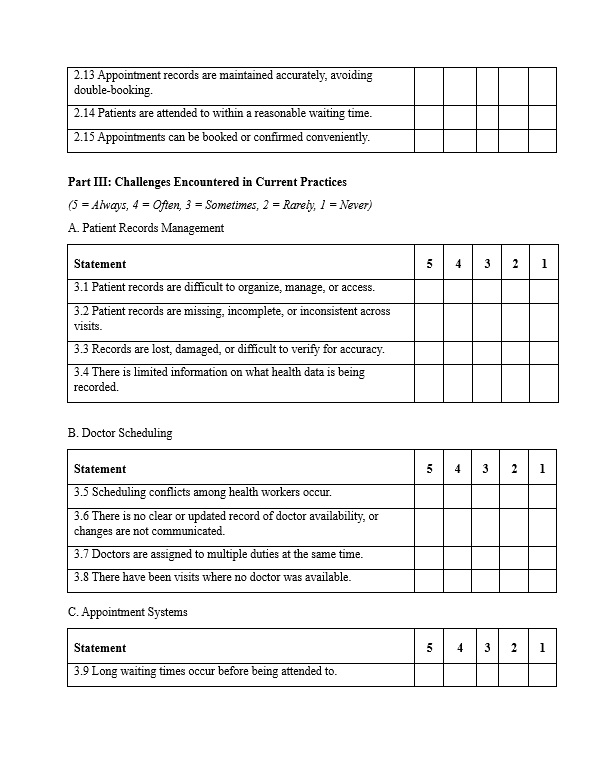
\includegraphics[width=0.95\textwidth]{3 survey(4).png}
\end{figure}

\begin{figure}[H]
    \caption*{Appendices A-8}
    \centering
    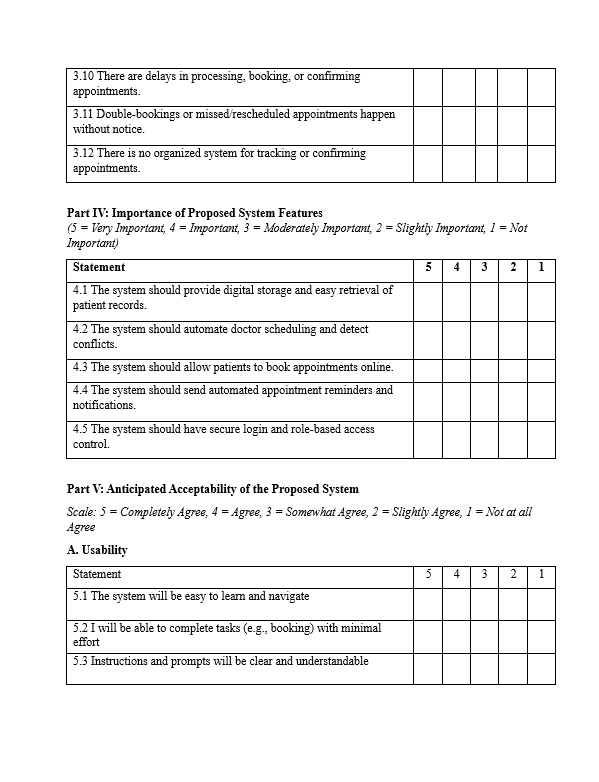
\includegraphics[width=0.95\textwidth]{4 survey(5).png}
\end{figure}

\begin{figure}[H]
    \caption*{Appendices A-9}
    \centering
    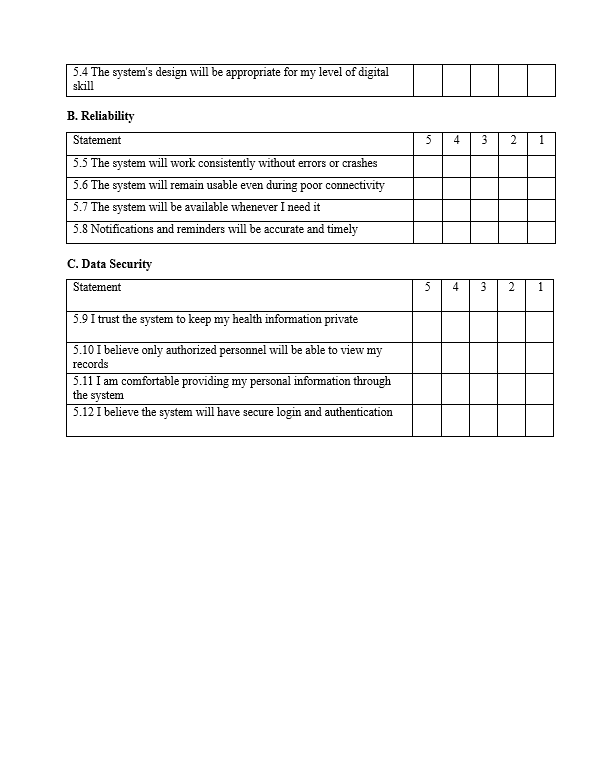
\includegraphics[width=0.95\textwidth]{5 survey(6).png}
\end{figure}

\begin{figure}[H]
    \caption*{Appendices A-12}
    \centering
    
\includegraphics[width=0.95\textwidth]{12}
\end{figure}

\begin{figure}[H]
    \caption*{Appendices A-13}
    \centering
    
\includegraphics[width=0.95\textwidth]{13}
\end{figure}

\nocite{ref70}
\nocite{ref71}
\nocite{ref72}
\end{document}